\documentclass[12pt,reqno]{amsart}
\usepackage{setspace}
\usepackage[inner=1in,outer=1in,tmargin=1in,bmargin=1in]{geometry}
\usepackage{mathtools}
\usepackage{amssymb}
\usepackage[utf8]{inputenc}
\usepackage[T1]{fontenc}
\usepackage[english]{babel}
\usepackage{parskip}
\usepackage{tensor}
\usepackage{hyperref}
\usepackage{amsmath}
\usepackage{afterpage}
\usepackage{tikz}
\usepackage{tikz-3dplot}
\usetikzlibrary{decorations.markings}
\usetikzlibrary{intersections}
\usetikzlibrary{arrows.meta}
\usepackage{lmodern}
\usepackage{graphicx}
\usepackage[capposition=bottom]{floatrow}
\usepackage{empheq}
\usepackage{amsthm}
\usepackage{lipsum}
\usepackage{cite}
\usepackage{cases}
\usepackage{hyperref}
\usepackage{pgfplots}
\pgfplotsset{compat=1.18}
\usepackage{enumitem}
\usepackage{pdfpages}
\usepackage{slashed}
\usepackage[colorinlistoftodos]{todonotes}
\usepackage{comment}
%\usepackage{mathrsfs}
\usepackage{dsfont}
\usepackage{comment}
\usepackage{mathtools}
\mathtoolsset{showonlyrefs}
\numberwithin{equation}{section}




%\usepackage{fancyhdr}
%\pagestyle{fancy}

\allowdisplaybreaks

\hypersetup{
	colorlinks,
	linkcolor={red!80!black},
	citecolor={blue!80!black},
	urlcolor={blue!80!black},
	linktoc=page
}

\usetikzlibrary{decorations.pathmorphing,calc}
\makeatletter








%Spyros

\newcommand{\bg}{\Box_{g}}
\newcommand{\T}{\mathcal{T}}
\renewcommand{\H}{\mathcal{H}}
\renewcommand{\Im}{\textnormal{Im}}
\newcommand{\ct}{\mathfrak{c}}
\newcommand{\tchi}{\Tilde{\chi}}
\newcommand{\add}{a_\delta}
\newcommand{\bd}{b_\eta}
\newcommand{\rr}{\mathcal{R}}

\renewcommand{\todo}[1]{$\clubsuit$ {\tt #1}}



\newcommand{\order}[1]{\mathcal{O}\left(#1\right)} %creates the O(x^y) term
\newcommand{\pminus}[1]{^{-#1}}

\newcommand{\ricci}[2]{\text{Ric}(#1, #2)}

%second fundamental form
\newcommand{\II}{I\hspace{-0.05cm}I}

%mathcal tangent
\newcommand{\tangt}{\mathcal{T}}

\newcommand{\diff}[1]{\frac{\dd}{\dd #1}}
\newcommand{\taux}{{\kappa(x,v)}}


%Kulkarni-Nomizu product
\makeatletter
\newcommand\incircbin
{%
  \mathpalette\@incircbin
}
\newcommand\@incircbin[2]
{%
  \mathbin%
  {%
    \ooalign{\hidewidth$#1#2$\hidewidth\crcr$#1\bigcirc$}%
  }%
}
\newcommand{\oland}{\incircbin{\land}}
\makeatother

%tangential part
%\def\tang{\ThisStyle{\abovebaseline[0pt]{\scalebox{-1}{$\SavedStyle\perp$}}}}

\def\division{\char'057}
\setlength{\unitlength}{.95pt}

\theoremstyle{definition}

\theoremstyle{plain}
\newtheorem{theorem}{Theorem}[section]
\newtheorem{lemma}[theorem]{Lemma}
\newtheorem{proposition}[theorem]{Proposition}
\newtheorem{hyp}{Hypothesis}
\newtheorem{corollary}[theorem]{Corollary}




\theoremstyle{definition}
\newtheorem{definition}[theorem]{Definition}




\theoremstyle{definition}
\newtheorem{question}[theorem]{Question}
\newtheorem{remark}[theorem]{Remark}
\newtheorem{example}[theorem]{Example}

\newtheorem{assumption}[theorem]{Assumption}


\newcommand{\ack}[1]{{\color{red}{{\bf #1}}}}
\newcommand{\vsp}{\vspace{0.3cm}}

\newcommand{\Abs}[1]{\Bigg\rvert #1 \Bigg\rvert}
\newcommand{\Norm}[1]{\Big\rVert #1 \Big\rVert}

\newcommand{\innerproduct}[2]{\langle #1, #2 \rangle}

\newcommand{\dd}{\text{d}}

\newcommand{\F}{\mathcal{F}}
\newcommand{\LR}{\mathcal{L}}

\newcommand{\R}{\mathbb{R}}

\def\C{\mathbb C}
\newcommand{\N}{\mathbb{N}}
\newcommand{\Cinf}{C^\infty}
\newcommand{\Cinfo}{C^\infty_0}

\newcommand{\sidenote}[1]{\marginpar{\ack{{\scriptsize #1}}}}
\newcommand{\ods}{\overline{d}^s}

\newcommand{\U}{\uu}
\newcommand{\G}{\mathcal{G}}
\newcommand{\B}{\mathcal{B}}
\newcommand{\magn}{\mathcal{H}}
\newcommand{\A}{\mathcal{A}}

\newcommand{\im}{\iota}
\newcommand{\I}{\boldsymbol{I}}
\newcommand{\J}{\boldsymbol{J}}
\newcommand{\Proj}{\boldsymbol{P}}
\newcommand{\bs}[1]{\boldsymbol{#1}}
\newcommand{\ola}{\overline{A}}
\newcommand{\olm}{\overline{M}}

\newcommand{\ww}{\Box_{A,Q}}

\newcommand{\n}{\mathcal{H}}
\newcommand{\sol}{\mathcal{S}}
\renewcommand{\U}{\uu}


\newcommand{\M}{\mathcal{M}}
\newcommand{\D}{\mathcal{D}}
\newcommand{\Ht}{\mathcal{H}_{\tau}}
\newcommand{\dg}{\D_\gamma}

\newcommand{\uu}{M}



%interior of a set
\newcommand{\intr}[1]{\operatorname{Int} #1}

\setlength{\parskip}{0pt}
\setlength{\parindent}{20pt}
%\onehalfspacing

\def\p{\partial}
\DeclareMathOperator{\supp}{supp}
\DeclareMathOperator{\id}{id}
\DeclareMathOperator{\GL}{\mathsf{GL}}
\providecommand{\HOX}[1]{\todo[noline]{#1}}
\providecommand{\TODO}[1]{\todo[inline]{#1}}

\pagestyle{headings}


\let\div\relax
\DeclareMathOperator{\div}{div}

\def\p{\partial}
\def\R{\mathbb R}
\DeclarePairedDelimiter{\norm}{\lVert}{\rVert}

\let\div\relax
\DeclareMathOperator{\div}{div}
\DeclareMathOperator{\vol}{vol}
\DeclarePairedDelimiter{\pair}{\langle}{\rangle}



\begin{document}


\begin{abstract}
We consider the inverse problem of recovering a potential $q$, depending on space and time, in the wave equation $(\Box_g+q)u=0$ on a Lorentzian manifold. We prove Lipschitz stability for a formally determined version of this problem under a \textit{null-cone foliation} assumption. As a consequence, we obtain uniqueness in the Lorentzian Calder\'on problem for $q$ under this assumption. Our approach is based on a modification of the Bukhgeim--Klibanov method using distorted plane waves.
\end{abstract}


\title[Stability for a Lorentzian inverse problem]{Stability for a formally determined Lorentzian inverse problem}

\author[S.FILIPPAS, L. OKSANEN]{Spyridon Filippas, Lauri Oksanen}

\address{Department of Mathematics and Statistics, University of Helsinki, PO BOX 68, 00014, HELSINKI, Finland}
\email {spyridon.filippas@helsinki.fi}

\address{Department of Mathematics and Statistics, University of Helsinki, PO BOX 68, 00014, HELSINKI, Finland}
\email {lauri.oksanen@helsinki.fi}


\maketitle
\tableofcontents

\section{Introduction}

\subsection{Setting}\label{sec:intro_setting}

We consider $(\M,g)$ a globally hyperbolic Lorentzian manifold of dimension $1+n$. We write $\Box_{g}$ for the Laplace-Beltrami operator on $\M$ defined by $\Box_{g}u= - \textnormal{div}_{g} \nabla^{g}u$. We consider as well a compactly supported potential $q \in C^\infty (\M ; \C ) $ with $\supp(q) \subset K$. We refer the reader to the Appendix~\ref{ap_lorentz} for facts in Lorentzian geometry used in this article.

The Lorentzian Calder\'on problem asks to recover the coefficients of a wave equation on a compact Lorentzian manifold with boundary from the Cauchy data of its solutions. We consider the operator $\Box_g+q$ where $q$ is a compactly supported potential. Our main result, Theorem~\ref{thm_main}, is Lipschitz stability for a formally determined inverse problem: the Cauchy data on $\partial\uu$ of one wave per leaf of a null-cone foliation determine $q$, with a Lipschitz estimate. The main novelty of this paper is the geometric condition under which this holds, the null-cone foliation assumption which we now state. 



\begin{assumption}[Null-cone foliation]
\label{assumption_null_cone_foliation}
We assume that there exists an open causal diamond $\mathcal{D} = I^+(p_-) \cap I^-(p_+)$ generated by two points $p_-, p_+ \in \M$, such that the following holds. There is a smooth future-directed timelike curve $\gamma \colon I \to \mathcal{D}$,
and an open neighbourhood $\uu$ of $K$ such that
\[
  K \subset \uu \Subset \mathcal{D},
  \qquad
  \overline{\uu} \cap \gamma(I) = \emptyset.
\]
For every $\tau \in I$, the \emph{regular part} of the future null
cone of $\gamma(\tau)$,
\[
  \mathcal{H}_\tau
  =
  \bigl(\partial J^+(\gamma(\tau)) \setminus \{\gamma(\tau)\}\bigr)
  \cap \mathcal{D},
\]
is a smooth null hypersurface, and the family
$\{\mathcal{H}_\tau\}_{\tau \in I}$ forms a smooth foliation of
\begin{equation}
    \label{def_of_dgamma}
\dg=\mathcal{D} \setminus \gamma(I).
\end{equation}
More precisely,
\[
  \dg = \bigsqcup_{\tau \in I} \mathcal{H}_\tau.
\]
and there exists a smooth function $f \colon \dg
\to I$ with $df \neq 0$ such that $\mathcal{H}_\tau = f^{-1}(\tau)$
for all $\tau \in I$.
\end{assumption}
Notice in particular the null condition,
\begin{equation}
\label{eq:null-cond}
g^{-1}(df,df) = 0  \textnormal{ on } \dg.
\end{equation}

\begin{figure}[ht]
\centering
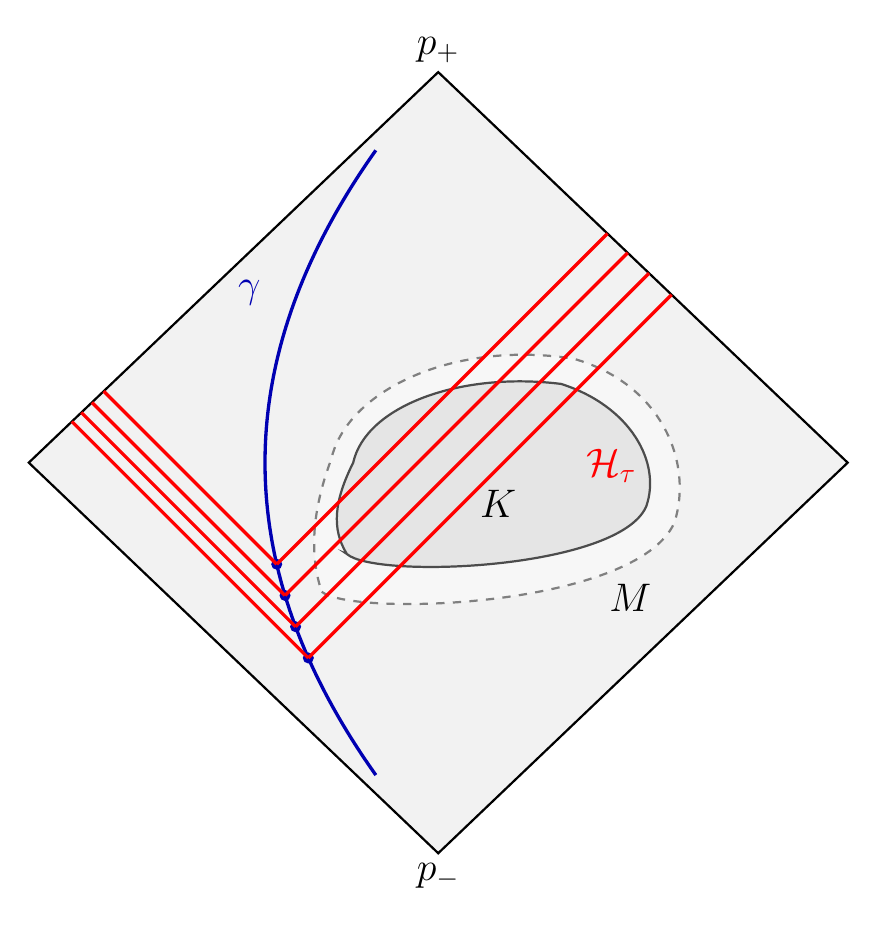
\begin{tikzpicture}[scale=0.8]

% -------------------------------------------------
% Causal diamond
% -------------------------------------------------
\fill[gray!10, draw=black, thick]
    (-1.5,0) -- (5,6.2) -- (11.5,0) -- (5,-6.2) -- cycle;

\node[above] at (5,6.2) {\Large $p_+$};
\node[below] at (5,-6.2) {\Large $p_-$};

% -------------------------------------------------
% Timelike curve gamma
% gamma(t) = (2.25 + 2.75 t^2, 6.2 t)
% -------------------------------------------------
\draw[blue!70!black, very thick, domain=-0.8:0.8, samples=100]
    plot ({2.25+2.75*\x*\x},{6.2*\x});

\node[blue!70!black] at (2,2.7) {\Large $\gamma$};

% -------------------------------------------------
% Neighborhood U
% -------------------------------------------------
\fill[white, opacity=0.45]
    (3.15,-2.05)
    .. controls (3.65,-2.45) and (8.15,-2.30) .. (8.75,-0.95)
    .. controls (9.05,0.0) and (8.55,1.25) .. (7.15,1.65)
    .. controls (5.25,1.95) and (3.55,1.15) .. (3.30,0.05)
    .. controls (3.00,-0.75) and (2.95,-1.45) .. cycle;

\draw[black!50, thick, dashed]
    (3.15,-2.05)
    .. controls (3.65,-2.45) and (8.15,-2.30) .. (8.75,-0.95)
    .. controls (9.05,0.0) and (8.55,1.25) .. (7.15,1.65)
    .. controls (5.25,1.95) and (3.55,1.15) .. (3.30,0.05)
    .. controls (3.00,-0.75) and (2.95,-1.45) .. cycle;

\node at (8.05,-2.15) {\Large $\uu$};

% -------------------------------------------------
% Compact set K
% -------------------------------------------------
\fill[black!10]
    (3.55,-1.45)
    .. controls (4.00,-1.85) and (7.85,-1.70) .. (8.30,-0.70)
    .. controls (8.55,0.0) and (8.05,0.90) .. (6.95,1.25)
    .. controls (5.35,1.45) and (3.85,0.90) .. (3.65,0.0)
    .. controls (3.35,-0.60) and (3.30,-1.05) .. cycle;

\draw[black!70, thick]
    (3.55,-1.45)
    .. controls (4.00,-1.85) and (7.85,-1.70) .. (8.30,-0.70)
    .. controls (8.55,0.0) and (8.05,0.90) .. (6.95,1.25)
    .. controls (5.35,1.45) and (3.85,0.90) .. (3.65,0.0)
    .. controls (3.35,-0.60) and (3.30,-1.05) .. cycle;

\node at (5.95,-0.65) {\Large $K$};

% -------------------------------------------------
% Exact points on gamma
% gamma(t) = (2.25 + 2.75 t^2, 6.2t)
% -------------------------------------------------

% t = -0.50
\coordinate (G1) at ({2.25+2.75*0.25},{6.2*(-0.50)});

% t = -0.42
\coordinate (G2) at ({2.25+2.75*0.42*0.42},{6.2*(-0.42)});

% t = -0.34
\coordinate (G3) at ({2.25+2.75*0.34*0.34},{6.2*(-0.34)});

% t = -0.26
\coordinate (G4) at ({2.25+2.75*0.26*0.26},{6.2*(-0.26)});

\fill[blue!70!black] (G1) circle (2.5pt);
\fill[blue!70!black] (G2) circle (2.5pt);
\fill[blue!70!black] (G3) circle (2.5pt);
\fill[blue!70!black] (G4) circle (2.5pt);

% -------------------------------------------------
% Future null cones
% Exactly 45 degrees
% Terminate exactly at the outer diamond
% -------------------------------------------------

% H_tau
\draw[red, very thick]
    (G1) -- (-0.81545,0.65295);
\draw[red, very thick]
    (G1) -- (8.70423,2.66673);

% H_tau'
\draw[red, very thick]
    (G2) -- (-0.66519,0.79629);
\draw[red, very thick]
    (G2) -- (8.34678,3.00768);

% H_tau''
\draw[red, very thick]
    (G3) -- (-0.49690,0.95680);
\draw[red, very thick]
    (G3) -- (8.00735,3.33145);

% H_tau'''
\draw[red, very thick]
    (G4) -- (-0.31060,1.13450);
\draw[red, very thick]
    (G4) -- (7.68593,3.63803);

% -------------------------------------------------
% Leaf label
% -------------------------------------------------
\node[red] at (7.75,-0.05) {\Large $\mathcal H_\tau$};

\end{tikzpicture}

\caption{The null-cone foliation of a neighborhood $\uu$ of the
compact set $K$ inside the causal diamond
$\D=I^+(p_-)\cap I^-(p_+)$. The timelike curve $\gamma$ joins $p_-$ to
$p_+$ and remains disjoint from $\overline{\uu}$. The family
$\{\mathcal H_\tau\}_{\tau\in I}$ foliates $\dg$.}
\label{fig:null_cone_foliation}
\end{figure}

\begin{remark}
Let us comment briefly on the geometric content of
Assumption~\ref{assumption_null_cone_foliation}.
The inclusion
\begin{equation}
    K \subset \U \Subset \D
\end{equation}
ensures that the compact set $K$ is contained in a relatively compact
causal diamond. In particular, all the geometric constructions below
can be carried out in a fixed causally bounded region.

The condition $\overline{\U}\cap\gamma(I)=\emptyset$
ensures that the neighborhood in which we work stays uniformly away
from the vertices of the null cones. This allows us to disregard the
singular behavior of the cones at their vertices.
For each $\tau\in I$, the set
\begin{equation}
    \n_\tau
    = \bigl(\partial J^+(\gamma(\tau)) \setminus \{\gamma(\tau)\}\bigr)
  \cap \mathcal{D}
\end{equation}
is assumed to be a smooth null hypersurface. This is not automatic on a
general Lorentzian manifold: null cones may develop conjugate points
and caustics, and their causal boundaries need not be smooth globally.
Thus, this condition amounts to assuming that the relevant portions of
the null cones are free of such singularities in $\mathcal{D}$.
\end{remark}

\begin{remark}[Global hyperbolicity of $\mathcal{D}$]\label{rem_D_globhyp}
The causal diamond $\mathcal{D}=I^+(p_-)\cap I^-(p_+)$ is globally
hyperbolic. It is causally convex: if $x,y\in\mathcal{D}$ and
$\lambda$ is a future-directed causal curve from $x$ to $y$, then
for any $z$ on $\lambda$ one has $p_-\ll x\leq z$, hence $p_-\ll z$,
and $z\leq y\ll p_+$, hence\footnote{This uses the chronological transitivity property: $x \ll y$ and $y \leq z$ implies $x \ll z$.}$z\ll p_+$, so $z\in\mathcal{D}$. For $x,y\in\mathcal{D}$, the diamond $J^+(x)\cap J^-(y)$ in
$\mathcal{D}$ equals the one in $\mathcal{M}$
hence is compact. As a consequence $\mathcal{D}$ is globally hyperbolic.
\end{remark}

\subsection{Results}

We begin with our result on the Lorentzian Calder\'on problem, which is simpler to state. It is a consequence of our main result, Theorem~\ref{thm_main}, a Lipschitz stability estimate for a formally determined inverse problem.

\subsubsection{The Lorentzian Calder\'on problem}

In the Lorentzian Calder\'on problem, only a compact Lorentzian manifold with boundary is given, and the data are the Cauchy data of the solutions on it.

Let $(\overline\uu,g)$ be a compact, time-oriented Lorentzian manifold of dimension $1+n$ with smooth boundary, and let $K\subset\uu$ be compact. For $q\in C^\infty(\overline\uu)$ with $\supp q\subset K$, the Cauchy data set of $\Box_g+q$ on $\uu$ is
\begin{equation}\label{eq_cds}
\mathcal C_q(\uu)=\bigl\{(u|_{\partial\uu},\partial_{\nu}u|_{\partial\uu}) : u\in C^\infty(\overline\uu),\ (\Box_g+q)u=0\text{ in }\uu\bigr\},
\end{equation}
where $\partial_\nu$ is the outward normal derivative of $u$ with respect to some fixed reference Riemannian metric on $\overline \uu$.
\begin{definition}[Null-cone extension]\label{def_extension}
A null-cone extension of $(\uu,g)$ is a globally hyperbolic Lorentzian manifold $(\M,\tilde g)$ of dimension $1+n$, together with an isometric, time-orientation preserving embedding $\overline\uu\subset\M$, such that Assumption~\ref{assumption_null_cone_foliation} holds for $(\M,\tilde g)$ and $K$, with $\uu$ as the neighbourhood of $K$.
\end{definition}

Thus a null-cone extension consists of $(\M,\tilde g)$, a causal diamond $\D$ with $\overline\uu\subset\D$, a timelike curve $\gamma$ in $\D$ with $\gamma(I)\cap\overline\uu=\emptyset$, and the function $f$ whose level sets are the future null cones of the points of $\gamma$, foliating $\D\setminus\gamma(I)$.

\begin{theorem}[Lorentzian Calder\'on problem]\label{thm_calderon}
Assume that $(\uu,g)$ has a null-cone extension. Let $q_1,q_2\in C^\infty(\uu)$ with $\supp q_j\subset K$. If $\mathcal C_{q_1}(\uu)\subset\mathcal C_{q_2}(\uu)$, then $q_1=q_2$.
\end{theorem}

The hypothesis is a condition on $(\uu,g)$ only, and the data are the Cauchy data sets, which depend only on $(\uu,g)$ and $q_j$. The extension is used only in the proof, where the $q_j$ are extended by zero.

\begin{remark}[Examples]\label{rem_examples}
Let $(N,h_N)$ be a complete Riemannian manifold, and let $\overline\uu$ be a compact domain with smooth boundary in the ultrastatic spacetime $(\R\times N,-dt^2+h_N)$. Assume that there is a point $x_0\in N$ outside the compact set $\pi_N(\overline\uu)$ such that $\exp_{x_0}\colon T_{x_0}N\to N$ is a diffeomorphism, where $\pi_N\colon\R\times N\to N$ is the projection. Then $(\uu,g)$ has a null-cone extension, by Lemma~\ref{lem:ultrastatic-foliation}. In particular, every compact domain with smooth boundary in Minkowski space has a null-cone extension.
\end{remark}


\subsubsection{Formally determined stability}\label{sec:intro_fd}

The quantities $K, \uu, \mathcal{D}, f$ are from now on fixed by Assumption~\ref{assumption_null_cone_foliation}. For $\tau\in I$ we write
 \begin{equation}
 \label{def_of_quantities}
     \varphi_{\tau} = f-\tau, \qquad \mathcal{H}_{\tau} = \{\varphi_{\tau}=0\}, \qquad Q_{\tau} = \{f>\tau\},\qquad L = -\nabla_g f .
 \end{equation}
Notice that since $f$ is defined on $\dg$, we have $Q_\tau\subset\dg$. The vector field $L$ is null, tangent to every leaf, and future-directed (see Lemma~\ref{lem_monotone}(c)).

To construct our plane waves in this Lorentzian setting, we need to define a notion of \textit{delta plane} supported on a null hypersurface $\n$. This is going to be a distribution on $\M$ supported on the null hypersurface $\n$. We refer to the appendix~\ref{ap_distrib_manifold} where we have collected some important facts about distributions on manifolds.

Let $\mathcal O\subset\M$ be open and let $\phi\in C^\infty(\mathcal O)$ be real with $d\phi \neq 0 $ on $\n=\{\phi=0\}$. We define the pullback distribution $\delta(\phi)=\phi^*(\delta_0) \in \mathcal{D}^\prime(\mathcal O) $ where $\delta_0$ is the Dirac distribution on the real line. This is a well defined distribution on $\mathcal O$, and as such acts on compactly supported densities. By using the natural density of $\M$, we can see $\delta(\phi)$ as a functional on $C^\infty_0(\mathcal O)$.

Even though this object is well defined, it is interesting to understand it in a more geometrically transparent way. More precisely, one would like to correlate this distribution with a notion of surface measure on $\n$. However, there is not a canonic way of integrating on a null hypersurface on a Lorentzian manifold, since the induced metric on $\n$ is degenerate. We can nevertheless relate $\delta(\phi)$ to a~\textit{Riemannian} surface measure. Indeed, we introduce an auxiliary Riemannian metric $h$ having the same density as $g$. Such a metric $h$ is given in Lemma~\ref{lem_aux_riem_metric}. Then, one can show as in~\cite[Theorem 6.1.5]{hormander1990} that in fact
\begin{equation}
    (\delta(\phi), w)=\int_\n \frac{w}{|\nabla_h \phi|_h} d \sigma_h,
\end{equation}
 where $d\sigma_h$ is the induced surface measure on $\n$ coming from \textit{the Riemannian metric } $h$. In other terms, we have the relationship
 \begin{equation}
     \delta(\phi)=\frac{d \sigma_h}{|\nabla_h \phi|_h}.
 \end{equation}

 We define as well the Heaviside function $H(\phi)$ associated to $\phi$ as $H(\phi)=\phi^*{H}$ where $H$ is the Heaviside function on $\R$. Using the chain rule~\eqref{eq_chain_rule} we get the expected relationship in coordinates between $\delta$ and $H$
 \begin{equation}
     \partial_jH(\phi)=\partial_j \phi\, \delta(\phi).
 \end{equation}

Throughout the article, $\nu$ will be the outward unit normal to $\partial\uu$ with respect to the auxiliary Riemannian metric $h$, and $\partial_\nu$ the corresponding normal derivative.

\bigskip


To define a distorted plane wave adapted to our geometric setting, we solve an inhomogeneous wave equation whose source is concentrated on one leaf $\mathcal H_\tau$ and localized by a cut-off $\chi$. For $x\in\dg$, the null generator of $\mathcal H_{f(x)}$ through $x$ is a null geodesic emanating from the vertex $\gamma(f(x))$ (see Section~\ref{sec_progressive_wave}). We will require that $\chi$ meets every such generator segment ending in $K$.

\begin{assumption}[On the sources]\label{assumption_sources}
We assume that $\chi\in C^\infty_c(\dg; [0,1])$ satisfies the following. For every $x\in K$ the segment of the null generator through $x$ from $\gamma(f(x))$ to $x$ meets $\{\chi>0\}$.
\end{assumption}

\begin{figure}[ht]
\centering
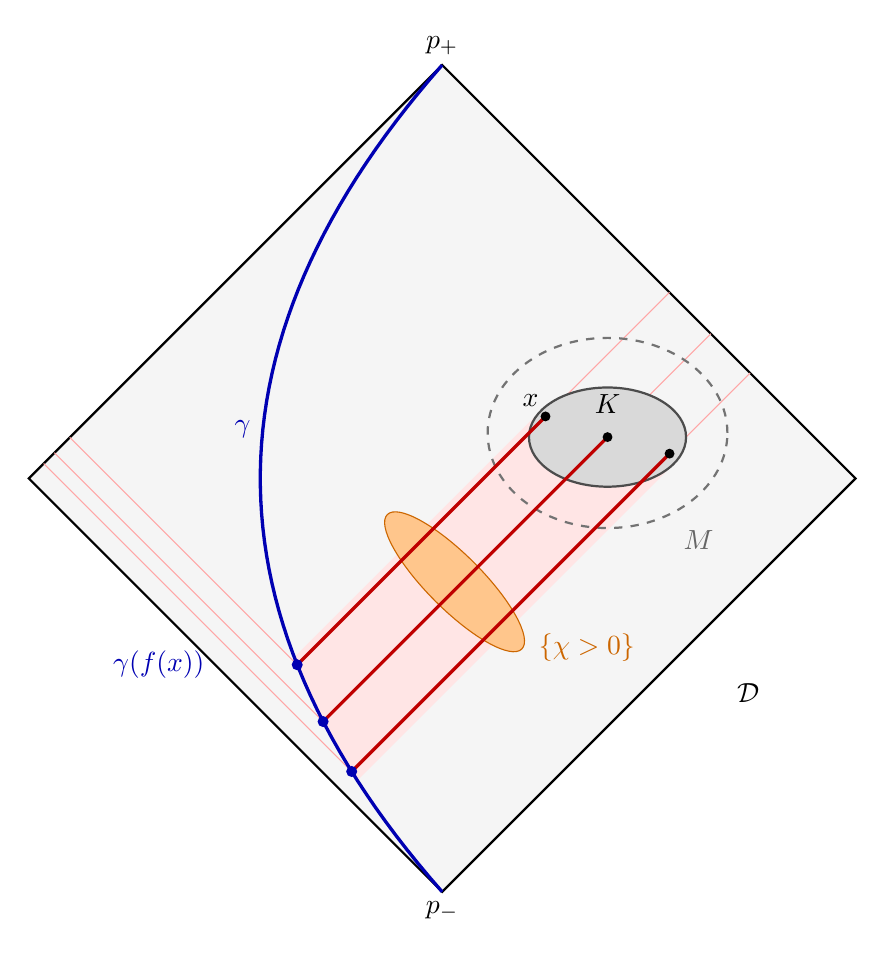
\begin{tikzpicture}[scale=1.05]
% causal diamond D, with p_- = (0,-5), p_+ = (0,5)
\fill[gray!8, draw=black, thick] (0,-5) -- (5,0) -- (0,5) -- (-5,0) -- cycle;
\node[below] at (0,-5) {$p_-$};
\node[above] at (0,5) {$p_+$};
\node at (3.7,-2.6) {$\mathcal D$};

% point x_1=(1.25,0.75), vertex gamma(f(x_1)) at s=-2.253
\coordinate (V1) at (-1.753,-2.253);\coordinate (X1) at (1.25,0.75);
\coordinate (R1) at (2.750,2.250);\coordinate (L1) at (-4.503,0.497);
% point x_2=(2.0,0.5), vertex gamma(f(x_2)) at s=-2.940
\coordinate (V2) at (-1.440,-2.940);\coordinate (X2) at (2.0,0.5);
\coordinate (R2) at (3.250,1.750);\coordinate (L2) at (-4.690,0.310);
% point x_3=(2.75,0.3), vertex gamma(f(x_3)) at s=-3.544
\coordinate (V3) at (-1.094,-3.544);\coordinate (X3) at (2.75,0.3);
\coordinate (R3) at (3.725,1.275);\coordinate (L3) at (-4.819,0.181);

% the region swept by the segments from gamma(f(x)) to x, x in K
\fill[red!10] (-1.789,-2.162) -- (1.194,0.821) -- (2.806,0.179) -- (-1.026,-3.653)
  -- plot[domain=-3.653:-2.162, samples=20] ({-2.2*(1-(\x/5)*(\x/5))},{\x}) -- cycle;

% leaves through x_1, x_2, x_3 (future null cones of their vertices)
\foreach \i in {1,2,3}
  \draw[red!35] (L\i) -- (V\i) -- (R\i);

% neighbourhood M of K, and K
\draw[black!55, thick, dashed] (2.0,0.55) ellipse[x radius=1.45, y radius=1.15];
\node[black!60] at (3.1,-0.75) {$\uu$};
\fill[black!15, draw=black!70, thick] (2.0,0.5) ellipse[x radius=0.95, y radius=0.6];
\node at (2,0.9) {$K$};

% the set {chi > 0}, outside the closure of M
\fill[orange!45, draw=orange!80!black, rotate around={-45:(0.15,-1.25)}]
  (0.15,-1.25) ellipse[x radius=1.15, y radius=0.33];
\node[orange!80!black] at (1.75,-2.05) {$\{\chi>0\}$};

% generator segments from gamma(f(x_i)) to x_i
\foreach \i in {1,2,3}
  \draw[red!75!black, very thick] (V\i) -- (X\i);
\foreach \i in {1,2,3}
  \fill (X\i) circle (1.7pt);
\node[above left, xshift=1pt] at (X1) {$x$};

% timelike curve gamma from p_- to p_+
\draw[blue!70!black, very thick, domain=-5:5, samples=60]
  plot ({-2.2*(1-(\x/5)*(\x/5))},{\x});
\node[blue!70!black, left] at (-2.2,0.6) {$\gamma$};
\foreach \i in {1,2,3}
  \fill[blue!70!black] (V\i) circle (1.9pt);
\node[blue!70!black, left, xshift=-30pt] at (V1) {$\gamma(f(x))$};
\end{tikzpicture}
\caption{For $x\in K$, the null generator segment from $\gamma(f(x))$ to $x$ (thick) is part of the leaf $\mathcal H_{f(x)}$ (light). These segments sweep out the shaded region and Assumption~\ref{assumption_sources} requires that each of them meets $\{\chi>0\}$.}
\label{fig:sources}
\end{figure}

Since such a  $\chi$ is compactly supported in $\dg$ one has in particular that $\supp(\chi)\cap\gamma(I)=\emptyset$. Any $\chi\in C^\infty_c(\U)$ with $\chi \geq 0$ and $\chi=1$ on $K$ satisfies Assumption~\ref{assumption_sources}, since $x$ itself lies on the segment. Lemma~\ref{lem_exterior_source} gives $\chi$ satisfying Assumption~\ref{assumption_sources} with $\supp\chi\cap\overline\uu=\emptyset$.

Global hyperbolicity and Proposition~\ref{prop_wave_lorentz} allow to define $V_{\tau} \in \D^\prime(\D)$ the unique solution of
\begin{equation}
 \label{eq_wave_lorentz}
\begin{cases}
    (\bg+q) V_{\tau}=\chi \delta^\prime(\varphi_\tau)  \quad \textnormal{in } \D,\\
    \supp (V_{\tau}) \subset J^+(\supp (\chi \delta^\prime(\varphi_\tau))).
    \end{cases}
\end{equation}

We prove in Section~\ref{sec_progressive_wave} that $V=V_\tau$ admits the progressive wave representation
\begin{equation}\label{eq_progressive_decomposition}
V=\alpha\delta(\varphi_\tau)+v\,H(\varphi_\tau)\qquad\text{in }\D,
\end{equation}
where $\alpha=\alpha_\tau$ and $v=v_{q,\tau}$ belong to $C^\infty(\D)$ and satisfy the system~\eqref{system_a_v}. The important feature of the coefficients $\alpha,v $  is that $\alpha$ solves a transport equation involving $\theta$ and $\chi$ and it is independent of $q$. On the other hand, $v$ solves a transport equation involving $\alpha$ and $q$.

Consider the set
\begin{equation}
\Gamma_\tau=\overline{Q_\tau}\cap\partial\uu.
\end{equation}
We define as well $\mathcal R\subset I$ the set of regular values of $f|_{\partial\uu}$. We restrict to $\tau\in\mathcal R$ because, for such $\tau$, $\mathcal H_\tau$ is transversal to $\partial\uu$. In particular, this will allow to integrate by parts in $Q_\tau\cap\uu$ (see Section~\ref{sec_carleman}). The restriction is harmless since by Sard's theorem, $I\setminus\mathcal R$ has measure zero.

Now for $\tau \in \mathcal R$ the traces of $V_\tau$ and $\partial_\nu V_\tau$ on $\partial\uu$ are well defined \cite[Theorem~8.2.4 and Corollary~8.2.7]{hormander1990} and one can define the map
\begin{equation}\label{eq_data_V}
\tilde{\mathcal L}:\ q\longmapsto\bigl(V_{q,\tau}|_{\Gamma_\tau},\ \partial_\nu V_{q,\tau}|_{\Gamma_\tau}\bigr)_{\tau\in\mathcal R}.
\end{equation}

It is however more convenient to work with smooth functions. Since $V=v$ on $Q_\tau$, $V=0$ on $\{\varphi_\tau<0\}$, and $\alpha$ does not depend on $q$, these data are equivalent to
\begin{equation}\label{eq_data_v}
\mathcal L:\ q\longmapsto\bigl(v_{q,\tau}|_{\Gamma_\tau},\ \partial_\nu v_{q,\tau}|_{\Gamma_\tau}\bigr)_{\tau\in\mathcal R},
\end{equation}
that is, $\tilde{\mathcal L}q_1=\tilde{\mathcal L}q_2$ if and only if $(\mathcal Lq_1)_\tau=(\mathcal Lq_2)_\tau$ for all $\tau\in\mathcal R$. Given two potentials $q_1,q_2$ we shall write $v_{j,\tau}=v_{q_j,\tau}$, $j \in \{1,2\}$, for the corresponding data used in $\mathcal{L}q_j$, and $w_\tau=v_{1,\tau}-v_{2,\tau}$.

Fix $A>0$, an integer $k\ge0$, and $[\tau_a,\tau_b]\subset I$ with $f(K)\subset[\tau_a,\tau_b]$. The integer $k$ is fixed large enough depending only on $n$ by~\eqref{bound_admissible}. A potential $q\in C^\infty(\M)$ is \textit{admissible} if
\begin{equation}
\label{def_of_admissible}
\supp q\subset K \textnormal{ and } \|q\|_{C^k}\le A.
\end{equation}
For admissible $q_1,q_2$ and $\tau\in\mathcal R$ we set
\begin{equation}\label{eq_data_E}
 E_\tau=|v_{1,\tau}-v_{2,\tau}|^2_{\Gamma_\tau}+|\partial_\nu v_{1,\tau}-\partial_\nu v_{2,\tau}|^2_{\Gamma_\tau}+|\nabla_h^{\tan} v_{1,\tau}-\nabla_h^{\tan}v_{2,\tau}|^2_{\Gamma_\tau},\qquad \mathcal E= \sqrt{\int_{\tau_a}^{\tau_b} E_\tau\,d\tau },
\end{equation}
where $|\cdot|_{\Gamma_\tau}$ is the $L^2$ norm on $\Gamma_\tau$ for the measure induced by $h$, and $\nabla_h^{\tan}$ is the tangential $h$-gradient on $\partial\uu$. Since $\nabla_h^{\tan}w_\tau$ is determined by $w_\tau|_{\Gamma_\tau}$, $\mathcal E$ is determined by $\mathcal Lq_1$ and $\mathcal Lq_2$.

\begin{theorem}[Lipschitz stability]\label{thm_main}
There is $C>0$, depending only on $A$ in~\eqref{def_of_admissible} and on the geometric quantities of Assumption~\ref{assumption_null_cone_foliation} such that for all admissible $q_1,q_2$
\[
\|q_1-q_2\|_{L^2(K)}\le C\mathcal E.
\]
In particular, if $(\mathcal Lq_1)_\tau=(\mathcal Lq_2)_\tau$ for almost every $\tau\in I$, then $q_1=q_2$.
\end{theorem}

\begin{remark}[Amount of data]\label{rem_data_count}
The data in Theorem~\ref{thm_main} are the Cauchy data of $w_\tau$ on $\Gamma_\tau$, for $\tau\in[\tau_a,\tau_b]$. They are functions on
\[
\{(\tau,y):\ \tau\in[\tau_a,\tau_b],\ y\in\Gamma_\tau\}\subset\R\times\partial\uu,
\]
a set of dimension $1+n$, the number of variables of $q$. So the problem is formally determined. As for $u$ and $\partial_tu$ in \cite{doi:10.1137/21M1400596,krishnan2023point}, both the Dirichlet and the Neumann trace enter. The data are small in three respects: there is one source per leaf, with the fixed cut-off $\chi$; $V_\tau=0$ on $\partial\uu\setminus\overline{Q_\tau}$, so only $\Gamma_\tau$ carries information; and only the leaves with $\tau\in[\tau_a,\tau_b]$ are used. By contrast, the Dirichlet-to-Neumann map, and the Cauchy data set \eqref{eq_cds}, are described by a Schwartz kernel on $\partial\uu\times\partial\uu$, which depends on $2n$ variables.
\end{remark}

In Theorem~\ref{thm_main}, everything but $q$ is known: the manifold $(\M,g)$, the diamond, the foliation and the sources. In terms of Cauchy data on $\partial\uu$, it gives the following.

\begin{corollary}[Formally determined version]\label{cor_fd_calderon}
Fix a null-cone extension of $(\uu,g)$ and $\chi$ as above. Let $q_1,q_2$ be admissible, and assume that $V_{q_1,\tau}$ and $V_{q_2,\tau}$ have the same Cauchy data on $\partial\uu$ for almost every $\tau\in[\tau_a,\tau_b]$. Then $q_1=q_2$. More generally, $\|q_1-q_2\|_{L^2(K)}\le C\mathcal E$, with $\mathcal E$ and $C$ as in Theorem~\ref{thm_main}.
\end{corollary}



So Theorem~\ref{thm_main}, applied with sources outside $\overline\uu$, is a formally determined Calder\'on-type result: the traces on $\partial\uu$ of one wave per leaf, sent from outside $\overline\uu$, determine $q$, with Lipschitz stability. Theorem~\ref{thm_calderon} follows, since the inclusion $\mathcal C_{q_1}(\uu)\subset\mathcal C_{q_2}(\uu)$ implies that these traces agree (see the proof of Theorem~\ref{thm_calderon} in Section~\ref{sec_proof_main}). This formally determined part cannot be singled out in terms of $(\overline\uu,g)$ alone. The waves $V_{q,\tau}$ are defined by sources outside $\overline\uu$, on the null cones of $\gamma$, so they depend on the extension. This is why Theorem~\ref{thm_calderon} is stated with the whole Cauchy data set.

\subsection{Previous literature}

For time-dependent potentials in Minkowski space, uniqueness goes back to \cite{stefanov1989uniqueness} for inverse scattering, and to \cite{ramm1991} for the Dirichlet-to-Neumann map on an infinite cylinder $\R\times\Omega$. Stability estimates of logarithmic type were obtained in \cite{ben-aicha2015}. These results use the full Dirichlet-to-Neumann map, which is overdetermined. The Boundary Control method \cite{belishev1988} is based on Tataru's unique continuation theorem for the wave equation across non-characteristic hypersurfaces \cite{tataru1995}. This theorem holds for coefficients depending real analytically on time, in particular for time-independent ones, and accordingly the method extends to time-dependent coefficients only in the real analytic case \cite{eskin2007}. For smooth coefficients, unique continuation may fail across hypersurfaces that are not pseudoconvex \cite{alinhac1983}.

On Lorentzian manifolds, Stefanov and Yang \cite{stefanov2018} showed that the light ray transform of $q$ is determined by the Dirichlet-to-Neumann map. This reduces uniqueness to the injectivity of the light ray transform, which is known in real analytic \cite{stefanov2017support} and in stationary or static \cite{feizmohammadi2021light} geometries; see also \cite{kian2019a,feizmohammadi2021b} for product geometries. Under curvature bounds that are stable under perturbations of the metric, the potential was recovered in \cite{alexakis2022}, by combining elements of the Boundary Control method with unique continuation along a pseudoconvex foliation; see also \cite{alexakis2023,gomes2025}.

Another line of research concerns metrics in a fixed conformal class, that is, $g=c\,g_0$ with $g_0$ known, and only the conformal factor $c$ is to be determined. In the elliptic case, the seminal result \cite{sylvester1987} recovers $c$ when $g_0$ is the Euclidean metric, and \cite{dos-santos-ferreira2009,dos-santos-ferreira2016,carstea2023} treat $g_0=dt^2+h$ under geometric conditions on $h$. Similar results for $g_0=-dt^2+h$ are given in \cite{kian2019a,feizmohammadi2021b}, and \cite{stefanov2018,alexakis2022} go beyond this product form. For $n\ge2$, determining a conformal factor is the same problem as determining a potential, see for instance \cite{alexakis2022}. In particular, Theorem~\ref{thm_calderon} also applies to conformal factors.

Oksanen, Rakesh and Salo recovered the metric itself, up to a diffeomorphism, also from formally determined data, first when one of the two metrics is the Minkowski metric \cite{oksanen2024rigiditylorentziancalderonproblem}, and then when one of them is close to it \cite{oksanen2026semiglobaluniquenesslorentziancalderon}. These are uniqueness results, and they rely on the proximity to the Minkowski metric. In the present paper the unknown is a potential. However, the metric $g$ is a general Lorentzian metric satisfying the null-cone foliation assumption, not assumed to be close to the Minkowski metric, and we prove Lipschitz stability. On the other hand, the Lorentzian Calder\'on problem is not solvable on certain noncompact domains \cite{oksanen2026counter}.

The Bukhgeim--Klibanov method \cite{bukhgeim1981global} gives uniqueness and Lipschitz stability for formally determined inverse problems by means of Carleman estimates; see \cite{imanuvilov2001,bellassoued2017book} for hyperbolic equations with time-independent coefficients. On Lorentzian manifolds, global Lipschitz stability for an inverse source problem from boundary observations was proved in \cite{takase2023}, also by means of Carleman estimates. Rakesh and Salo \cite{rakesh2020fixed,rakesh2020two} used incoming plane waves in this method, for fixed angle scattering. Krishnan, Rakesh and Senapati \cite{doi:10.1137/21M1400596} modified it further to recover coefficients depending on space and time in Minkowski space, from a formally determined family of incoming plane waves, one for each delay, carried by the null hyperplanes $\{t=\tau+x\cdot\omega\}$; see also \cite{krishnan2023point} for point sources. We build on \cite{doi:10.1137/21M1400596}: our proof is a modification of the Bukhgeim--Klibanov method with distorted plane waves, as in \cite{doi:10.1137/21M1400596}, but in a general Lorentzian setting. One key new ingredient is the null-cone foliation assumption, under which the null hyperplanes of \cite{doi:10.1137/21M1400596} are replaced by the leaves of a null-cone foliation.

\subsection{Organization of the paper}

In Section~\ref{sec_progressive_wave} we prove a monotonicity lemma for the null-cone foliation and the progressive wave representation of $V_\tau$. Section~\ref{sec_carleman} is devoted to the Carleman estimate near a null cone, which is the main technical tool. In Section~\ref{sec_proof_main} we prove Theorem~\ref{thm_main}, and then Theorem~\ref{thm_calderon} by a gluing argument. Appendix~\ref{ap_lorentz} recalls facts from Lorentzian geometry, constructs the auxiliary metric $h$, and verifies Assumption~\ref{assumption_null_cone_foliation} in ultrastatic spacetimes. Appendix~\ref{ap_distrib_manifold} recalls facts on distributions on manifolds.




\section{Progressing-wave representation}
\label{sec_progressive_wave}

Given a null hypersurface $\n$, at each point $p \in \n $ the tangent space $T_p(\n)$ contains a null vector which is unique up to multiplication by a non zero scalar (see for instance~\cite[Lemma 28]{oneill1983}). We fix once and for all the vector field $L$ by
\begin{equation}
    \label{def_of_null_vector_L}
    L=-\nabla_g f.
\end{equation}
Then, $L$ is a smooth null vector field on $\dg$, tangent to every leaf $\mathcal H_\tau$, $\tau\in I$. Its integral curves are called the \textit{null generators} of the leaves. They are null geodesics since
$$
\nabla_LL=\frac12\nabla_g\bigl(g(\nabla f,\nabla f)\bigr)=0.
$$
We write
\begin{equation}
    P=\bg+q,
  \qquad
  \theta=\Box_g\varphi_\tau=\Box_gf,
  \label{eq:phi}
\end{equation}
where we recall that $\phi_\tau$ is defined in~\eqref{def_of_quantities}. Note that $\theta$ does not depend on $\tau$.






\subsection{A monotonicity lemma}




\begin{lemma}\label{lem_monotone}
Under Assumption~\ref{assumption_null_cone_foliation}, the following hold.
\begin{enumerate}[label=(\alph*),leftmargin=*]
\item (Level sets) For every $s\in I$,
\begin{equation}\label{eq:levelsets}
J^+(\gamma(s))\cap\dg=\{f\ge s\},
\qquad
I^+(\gamma(s))\cap\dg=\{f>s\}.
\end{equation}

\item (Monotonicity) Let $x,y\in\dg$. Then
\begin{equation}\label{eq:mono}
y\in J^+(x)\ \Longrightarrow\ f(y)\ge f(x),
\qquad
y\in I^+(x)\ \Longrightarrow\ f(y)>f(x).
\end{equation}
In particular, for every $\tau\in I$,
\begin{equation*}
J^+(\Ht)\cap\dg\subset\{f\ge\tau\}.
\end{equation*}
\item (Time orientation) The vector field $L=-\nabla_gf$ is future-directed.
\end{enumerate}
\end{lemma}

\begin{proof}
We use the following standard facts on the globally hyperbolic manifold $\M$ \cite{oneill1983}. For every $p\in\M$, the set $J^+(p)$ is closed and the set $I^+(p)$ is open. Moreover, the push-up property holds (see the footnote in Remark~\ref{rem_D_globhyp}): for $x,y,z\in\M$,
\begin{equation}\label{eq:pushup}
x\ll y\le z
\quad\text{or}\quad
x\le y\ll z
\qquad\Longrightarrow\qquad
x\ll z.
\end{equation}
Finally, since $\gamma$ is a future-directed timelike curve,
\begin{equation}\label{eq:gamma_order}
\gamma(s)\ll\gamma(s')\qquad\text{for } s<s'.
\end{equation}

(a) Let $x\in\dg$ and set $\sigma=f(x)$. By Assumption~\ref{assumption_null_cone_foliation},
\begin{equation*}
x\in\mathcal H_\sigma\subset\partial J^+(\gamma(\sigma)).
\end{equation*}
Since $J^+(\gamma(\sigma))$ is closed, its boundary is contained in it. Since $I^+(\gamma(\sigma))$ is open and contained in $J^+(\gamma(\sigma))$, it does not meet $\partial J^+(\gamma(\sigma))$. Hence
\begin{equation}\label{eq:AB}
\gamma(\sigma)\le x
\qquad\text{and}\qquad
\gamma(\sigma)\not\ll x.
\end{equation}
Now fix $s\in I$ and compare $\sigma$ with $s$.

If $\sigma>s$, then \eqref{eq:gamma_order} and \eqref{eq:AB} give
\begin{equation*}
\gamma(s)\ll\gamma(\sigma)\le x,
\end{equation*}
so $\gamma(s)\ll x$ by \eqref{eq:pushup}. In particular $\gamma(s)\le x$.

If $\sigma=s$, then $\gamma(s)\le x$ and $\gamma(s)\not\ll x$, by \eqref{eq:AB}.

If $\sigma<s$, then $\gamma(s)\not\le x$. Indeed, otherwise
\begin{equation*}
\gamma(\sigma)\ll\gamma(s)\le x,
\end{equation*}
and \eqref{eq:pushup} gives $\gamma(\sigma)\ll x$, which contradicts \eqref{eq:AB}. A fortiori, $\gamma(s)\not\ll x$.

Thus
\begin{equation*}
\gamma(s)\le x\iff f(x)\ge s,
\qquad
\gamma(s)\ll x\iff f(x)>s,
\end{equation*}
which is \eqref{eq:levelsets}.

(b) Let $x,y\in\dg$ with $y\in J^+(x)$, and set $s=f(x)$. By (a), $\gamma(s)\le x$, hence
\begin{equation*}
\gamma(s)\le x\le y.
\end{equation*}
So $\gamma(s)\le y$, and $f(y)\ge s$ by (a). If moreover $y\in I^+(x)$, then
\begin{equation*}
\gamma(s)\le x\ll y,
\end{equation*}
so $\gamma(s)\ll y$ by \eqref{eq:pushup}, and $f(y)>s$ by (a). Finally, if $y\in J^+(\Ht)\cap\dg$, then $y\in J^+(x)$ for some $x\in\Ht$, and $f(y)\ge f(x)=\tau$.

(c) Let $x\in\dg$ and let $Y\in T_x\M$ be future-directed timelike. Since $\dg$ is open, there is a future-directed timelike curve $c\colon[0,\delta)\to\dg$ with $c(0)=x$ and $\dot c(0)=Y$. For $0<t<\delta$ we have $c(t)\in I^+(x)$, so $f(c(t))>f(x)$ by (b). Hence
\begin{equation*}
df(Y)=\frac{d}{dt}f(c(t))\Big|_{t=0}\ge0.
\end{equation*}
The vector $\nabla_gf$ is normal to the null hypersurfaces $\mathcal H_\tau$, so it is null, and it is nonzero since $df\ne0$. A nonzero null vector is not orthogonal to a timelike vector, so $df(Y)=g(\nabla_gf,Y)\ne0$. Therefore
\begin{equation*}
g(L,Y)=-df(Y)<0,
\end{equation*}
and the null vector $L$ is future-directed.
\end{proof}
\begin{remark}[The whole diamond is foliated]\label{rem_whole_diamond}
It is important that the null cones foliate the whole of $\dg$, and not only a neighbourhood of $\overline\uu$, since the sources may lie outside $\overline\uu$. Lemma~\ref{lem_monotone} then allows to compare the values of $f$ at any two causally related points of $\dg$, wherever they are. In particular, a wave sent from the leaf $\mathcal H_\tau$ stays in $\{f\ge\tau\}$.
\end{remark}

\subsection{The progressive wave expansion}

We prove a progressive wave expansion property (like \cite[Proposition 1.2]{doi:10.1137/21M1400596}). Let $\Phi_s$ be the flow of $L$ on $\dg$. Since every leaf is null, $L$ is tangent to all leaves, and the generator through $x\in\dg$ is the null geodesic from the vertex $\gamma(f(x))$ to $x$. The following identity is the key calculation.

\begin{lemma}
\label{lem:key}
Let $\alpha,v\in C^\infty(\dg)$. Then, in $\dg$,
\begin{equation}
\begin{aligned}
  P\bigl(\alpha\,\delta(\varphi)+v\,H(\varphi)\bigr)
  ={}&
  \bigl(2L(\alpha)+\theta\alpha\bigr)\delta'(\varphi)
  \\
  &+
  \bigl(P\alpha+2L(v)+\theta v\bigr)\delta(\varphi)
  +
  (Pv)H(\varphi).
\end{aligned}
\label{eq:key}
\end{equation}
\end{lemma}

\begin{proof}
Since $\Box_g=-\div_g\nabla$, $g(\nabla\varphi,\nabla\varphi)=0$, $L=-\nabla\varphi$ and $\theta=\Box_g\varphi$, for $a\in C^\infty(\dg)$ and $F\in\mathcal D'(\R)$ we have
\begin{equation}\label{eq:PaF}
P\bigl(a\,F(\varphi)\bigr)=F(\varphi)\,Pa+F'(\varphi)\,\bigl(2L(a)+\theta a\bigr).
\end{equation}
In particular
\begin{equation}
  \Box_gH(\varphi)=\theta\,\delta(\varphi),
  \qquad
  \Box_g\delta(\varphi)=\theta\,\delta'(\varphi).
  \label{eq:box-H-delta}
\end{equation}
With $F=H$ and $F=\delta$, \eqref{eq:PaF} yields
\begin{equation}
  P(v\,H(\varphi))
  =
  (Pv)\,H(\varphi)
  +
  (2L(v)+\theta v)\,\delta(\varphi),
  \label{eq:PvH}
\end{equation}
and
\begin{equation}
  P(\alpha\,\delta(\varphi))
  =
  (P\alpha)\,\delta(\varphi)
  +
  (2L(\alpha)+\theta\alpha)\,\delta'(\varphi).
  \label{eq:Palpha}
\end{equation}
Adding \eqref{eq:PvH} and \eqref{eq:Palpha} proves \eqref{eq:key}.
\end{proof}


\begin{proposition}
\label{prop_prog_wave}
Let $V$ be the unique solution of~\eqref{eq_wave_lorentz}. Then, there exist functions $\alpha,v\in C^\infty(\mathcal{D})$, with $\alpha$ vanishing near $\gamma(I)$,
such that
\begin{equation}
  V=\alpha\,\delta(\varphi)+v\,H(\varphi)
  \qquad\text{in }\mathcal{D}.
  \label{eq:main}
\end{equation}
Moreover, $\alpha$ satisfies
\begin{equation}
  2L(\alpha)+\theta\alpha=\chi
  \qquad\text{in }\dg,
  \label{eq:alpha}
\end{equation}
and there is $\delta_\alpha>0$ such that
\begin{equation}
  \alpha\ge\delta_\alpha\qquad\text{on }K.
  \label{eq:alpha-lower}
\end{equation}
\end{proposition}

\begin{proof}
\textbf{1. The ansatz and the transport equations.}
We look for a parametrix of the form
\begin{equation}\label{def_of_parametrix_r}
R_\infty=\alpha\,\delta(\varphi)+\widetilde v\,H(\varphi),
\qquad
\widetilde v\sim\sum_{k\ge0}w_k\,\varphi^k\quad\text{near }\Ht,
\end{equation}
with smooth functions $\alpha,w_0,w_1,\dots$, such that $PR_\infty-\chi\,\delta'(\varphi)$ is smooth. Then $V-R_\infty$ solves a wave equation with a smooth source, so it is smooth.

To find the equations for $\alpha$ and the $w_k$, let
\begin{equation*}
v_N=\sum_{k=0}^Nw_k\varphi^k .
\end{equation*}
Since $L\varphi=0$, \eqref{eq:PaF} gives
\begin{equation*}
P(w_k\varphi^k)=\varphi^kPw_k+k\varphi^{k-1}(2Lw_k+\theta w_k),
\qquad
(2L+\theta)v_N=\sum_{k=0}^N\varphi^k(2L+\theta)w_k .
\end{equation*}
As $\varphi^k\delta(\varphi)=0$ for $k\ge1$, Lemma~\ref{lem:key} gives
\begin{equation}\label{eq:ansatz}
\begin{aligned}
&P\bigl(\alpha\,\delta(\varphi)+v_N\,H(\varphi)\bigr)-\chi\,\delta'(\varphi)\\
&\quad=(2L\alpha+\theta\alpha-\chi)\,\delta'(\varphi)+(2Lw_0+\theta w_0+P\alpha)\,\delta(\varphi)\\
&\qquad+\sum_{k=1}^N\varphi^{k-1}\bigl(k(2Lw_k+\theta w_k)+Pw_{k-1}\bigr)H(\varphi)+\varphi^N(Pw_N)\,H(\varphi).
\end{aligned}
\end{equation}
So we impose the transport equations
\begin{equation}\label{eq:recursion}
\left\{
\begin{aligned}
&2L\alpha+\theta\alpha=\chi,\\
&2Lw_0+\theta w_0=-P\alpha,\\
&k\,(2Lw_k+\theta w_k)=-Pw_{k-1},\qquad k\ge1.
\end{aligned}
\right.
\end{equation}
Then only the last term of \eqref{eq:ansatz} remains. In particular,
\begin{equation}\label{eq:Pwk}
Pv_N=\varphi^N\,Pw_N .
\end{equation}
This error is only in $C^{N-1}$ and will be removed by letting $N\to\infty$ via Borel's theorem.

\medskip\noindent
\textbf{2. Solving the transport equations on all leaves.}
Each equation in \eqref{eq:recursion} has the form
\begin{equation*}
2La+\theta a=b,
\end{equation*}
with $b$ given by the previous equations. Since $L$ is tangent to the leaves, this is an ODE along each null generator. We solve it on every generator of every leaf $\mathcal H_s$, $s\in I$ and the solutions are then defined on all of $\dg$. This is important since $Pa$ involves derivatives of $a$ in directions transversal to $\mathcal H_\tau$.

Let $\lambda\colon(s_0,s_1)\to\dg$ be a generator, with $\dot\lambda=L\circ\lambda$ and $\lambda(s)$ tending to its vertex as $s\to s_0$. For $b$ vanishing near $\gamma(I)$, the unique solution along $\lambda$ that vanishes near the vertex is
\begin{equation}
  a(\lambda(s))
  =
  \frac{1}{2}
  \int_{s_0}^{s}
  b(\lambda(\sigma))
  \exp\!\left(
  -\frac{1}{2}\int_\sigma^s\theta(\lambda(r))\,dr
  \right)
  d\sigma .
  \label{eq:alpha-explicit}
\end{equation}
It is smooth on $\dg$, by smooth dependence of the flow of $L$ on the initial point.

It remains to check that the right-hand sides vanish near \textit{a whole neighbourhood} of $\gamma(I)$ in $\mathcal{D}$. By \eqref{eq:alpha-explicit}, $a(x)$ depends only on $b$ along the generator segment from $\gamma(f(x))$ to $x$. By Lemma~\ref{lem_monotone}, the points $y$ of this segment satisfy
\begin{equation}\label{eq:segment}
\gamma(f(x))\le y\le x .
\end{equation}
Let $s\in I$. Since $\M$ is globally hyperbolic, there is $\varepsilon>0$ such that
\begin{equation*}
J^+(\gamma(s-\varepsilon))\cap J^-(\gamma(s+\varepsilon))\cap\supp\chi=\emptyset .
\end{equation*}
Let
\begin{equation*}
\mathcal U_s=I^+(\gamma(s-\varepsilon))\cap I^-(\gamma(s+\varepsilon)),
\end{equation*}
an open neighbourhood of $\gamma(s)$ on which $\chi=0$. If $x\in\mathcal U_s\cap\dg$, then $f(x)>s-\varepsilon$ by Lemma~\ref{lem_monotone}(a). So, by \eqref{eq:segment}, every point $y$ of the generator segment to $x$ satisfies
\begin{equation*}
\gamma(s-\varepsilon)\ll\gamma(f(x))\le y\le x\ll\gamma(s+\varepsilon),
\end{equation*}
and hence $y\in\mathcal U_s$. Now $\alpha$ is determined by~\eqref{eq:alpha-explicit} for $b=\chi$ and it vanishes in $\cup_{s \in I} \mathcal U _s$ which is a neighbourhood of $\gamma(I)$. Moreover, the lower bound~\eqref{eq:alpha-lower} is an immediate consequence of the same formula
\begin{equation*}
\alpha(x)=\frac12\int_{s_0}^{0}\chi(\lambda(\sigma))\exp\Bigl(-\frac12\int_\sigma^0\theta(\lambda(r))\,dr\Bigr)d\sigma,
\end{equation*}
combined with the assumption~\ref{assumption_sources} on $\chi$. Indeed, since each generator meets the set $\{\chi >0\}$ we have that $\alpha(x)>0$ for all $x \in K$ and hence the lower bound by compactness.



Once $\alpha$ is constructed the subsequent $w_k$ are determined by solving the transport equations~\eqref{eq:recursion}. They vanish near $\gamma(I)$, and we extend them by zero to $\D$. In the same way, they vanish in the open set $\dg\setminus J^+(\supp\chi)$: by \eqref{eq:segment}, the generator segment to a point $x$ of this set lies in $J^-(x)$, hence in this set. Thus
\begin{equation*}
\supp\alpha\cup\bigcup_{k\ge0}\supp w_k\subset J^+(\supp\chi).
\end{equation*}



\medskip\noindent
\textbf{3. The parametrix.}
Since $d\varphi=df\neq0$, $\varphi$ can be used as a local coordinate near $\Ht$. By Borel's theorem~\cite[Theorem 1.2.6]{hormander1990}, applied in the variable $\varphi$, there is a function $\widetilde v_0$, smooth in a neighbourhood $\mathcal O$ of $\Ht$ in $\dg$, with prescribed Taylor coefficients in $\varphi$:
\begin{equation}
  \widetilde v_0-\sum_{k<N}w_k\varphi^k\in\varphi^N\,C^\infty(\mathcal O)\qquad\text{for every }N .
  \label{eq:borel}
\end{equation}
The function $\widetilde v_0$ is not yet what we need since it is defined only in $\mathcal O$, and only its Taylor coefficients on $\Ht$ are prescribed. We use a cut-off to extend to the whole $\mathcal D$.

Let $\mathcal N\subset\D$ be an open neighbourhood of $\gamma(I)$ on which all $w_k$ vanish. We pick $\vartheta\in C^\infty(\D)$ with
\begin{equation*}
\vartheta=1\quad\text{near }\Ht\setminus\mathcal N,
\qquad
\supp\vartheta\subset\mathcal O .
\end{equation*}
Since $\supp\vartheta$ is closed in $\D$ and does not meet $\gamma(I)$, $\vartheta$ vanishes near $\gamma(I)$. Let $\widetilde v=\vartheta\,\widetilde v_0$, extended by zero to $\D$. Then
\begin{equation*}
\widetilde v\in C^\infty(\D),
\qquad
\widetilde v=0\quad\text{near }\gamma(I).
\end{equation*}
The cut-off does not change the Taylor expansion on $\Ht$, so $\widetilde v$ still satisfies \eqref{eq:borel} near $\Ht$. By \eqref{eq:borel} and \eqref{eq:Pwk},
\begin{equation*}
P\widetilde v\in\varphi^NC^\infty\quad\text{near }\Ht,\ \text{for every }N,
\end{equation*}
that is, $P\widetilde v$ vanishes to infinite order on $\Ht=\{\varphi=0\}$. Now recalling that $R_\infty=\alpha \delta(\phi)+\tilde{v}H(\phi)$ Lemma~\ref{lem:key} gives
\begin{equation}
  F_\infty
  =
  PR_\infty-\chi\,\delta'(\varphi)
  =
  (P\widetilde{v})\,H(\varphi)
  \in C^\infty(\mathcal{D}).
  \label{eq:Finfty}
\end{equation}
The term $F_\infty$ is smooth because $P\widetilde v$ vanishes to infinite order on $\{\varphi=0\}$, and $F_\infty=0$ near $\gamma(I)$, since $\widetilde v=0$ there.

\medskip\noindent
\textbf{4. The smooth remainder.}
Set
\begin{equation}
  W=V-R_\infty,
  \qquad\text{so that}\qquad
  PW=-F_\infty\in C^\infty(\D)
  \label{eq:W}
\end{equation}
by \eqref{eq_wave_lorentz} and \eqref{eq:Finfty}. Since $\D$ is globally hyperbolic, it has a Cauchy temporal function $t_{\D}$. Let
\begin{equation*}
C=\supp\chi\cup\{\gamma(\tau)\},
\end{equation*}
a compact set, choose $t_0<\min_Ct_{\D}$, and let
\begin{equation*}
\Sigma=\{t_{\D}=t_0\},
\end{equation*}
an initial spacelike Cauchy hypersurface in the past of $C$. Since $t_{\D}$ increases along future-directed causal curves,
\begin{equation*}
J^+(C)\subset\{t_{\D}\ge\min_Ct_{\D}\},
\end{equation*}
so $J^+(C)$ does not meet the neighbourhood $\{t_{\D}<\min_Ct_{\D}\}$ of $\Sigma$. Now:
\begin{equation*}
\begin{aligned}
&\supp V\subset J^+(\supp(\chi\,\delta'(\varphi)))\subset J^+(C)&&\text{by \eqref{eq_wave_lorentz}},\\
&\supp\alpha\subset J^+(\supp\chi)\subset J^+(C)&&\text{by Step~2},\\
&\supp\bigl(\widetilde v\,H(\varphi)\bigr)\subset\overline{\{f\ge\tau\}}\subset J^+(\gamma(\tau))\subset J^+(C)&&\text{by Lemma~\ref{lem_monotone}(a)}.
\end{aligned}
\end{equation*}
Hence
\begin{equation*}
W=V-\alpha\,\delta(\varphi)-\widetilde v\,H(\varphi)=0\quad\text{near }\Sigma,
\end{equation*}
so $W$ solves $PW=-F_\infty$ with zero Cauchy data on $\Sigma$ and a smooth source. By well-posedness of the Cauchy problem we get that it is the unique smooth solution of this wave equation and in particular
\begin{equation}
  W\in C^\infty(\D).
  \label{eq:W-smooth}
\end{equation}

\medskip\noindent
\textbf{5. Conclusion.}
By \eqref{eq_wave_lorentz}, $\supp V\subset J^+(\supp\chi\cap\Ht)$, so Lemma~\ref{lem_monotone}(b) gives
\begin{equation*}
\supp V\cap\dg\subset\{\varphi\ge0\}.
\end{equation*}
By construction, $\supp R_\infty\subset\{\varphi\ge0\}$. So the smooth function $W=V-R_\infty$ vanishes on $\{\varphi<0\}$, that is,
\begin{equation*}
W=W\,H(\varphi).
\end{equation*}
Going back to $V=R_\infty+W$, we obtain
\begin{equation*}
V=\alpha\,\delta(\varphi)+v\,H(\varphi),\qquad v=\widetilde v+W\in C^\infty(\D),
\end{equation*}
which finishes the proof of~\eqref{eq:main}.
\end{proof}

\begin{figure}[ht]
\centering
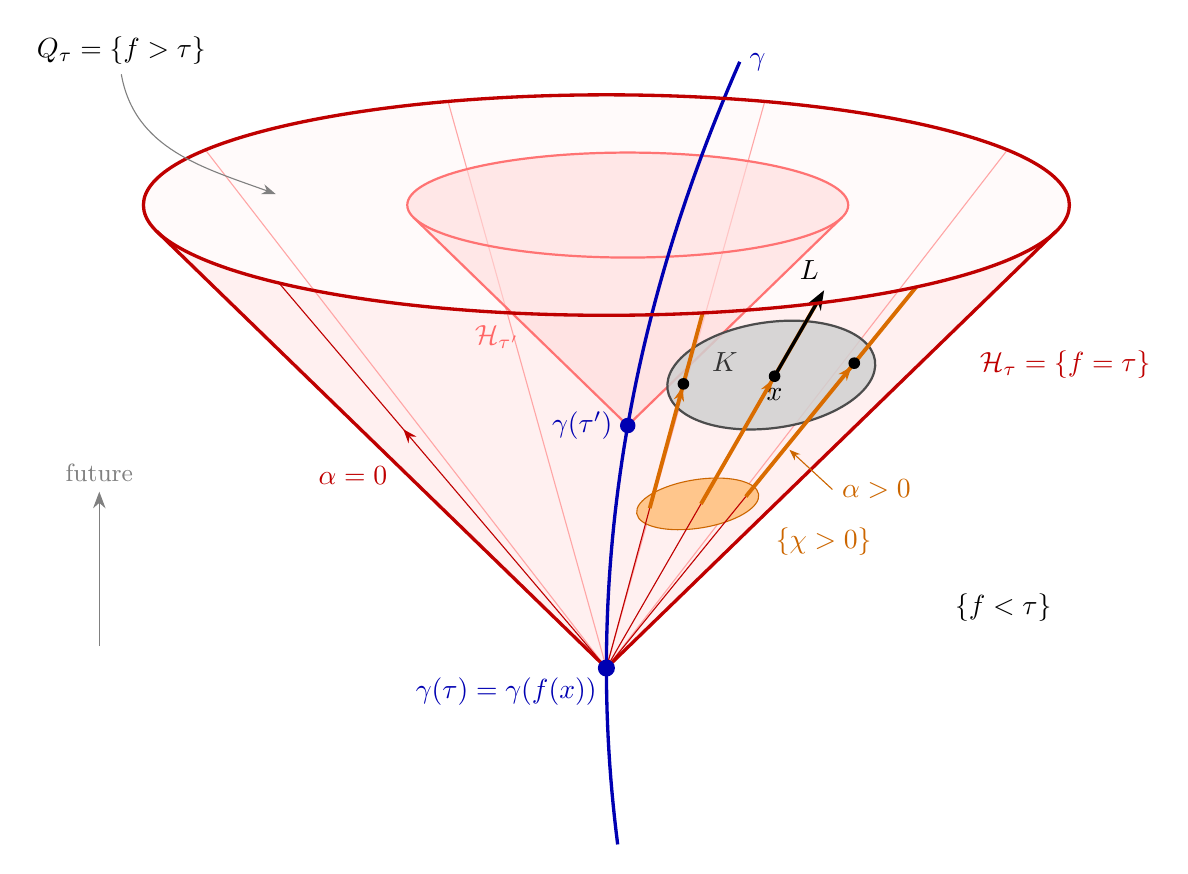
\begin{tikzpicture}[scale=1.4,
  gen/.style={red!75!black, thin},
  genback/.style={red!35, thin},
  flow/.style={postaction={decorate},
    decoration={markings, mark=at position 0.62 with {\arrow{Stealth[length=5pt]}}}}]

% parameters: outer leaf H_tau, vertex gamma(tau) at the origin,
% cross-section at height \Hh is an ellipse with radii \Ra, \Rb
\def\Ra{4.2}\def\Hh{4.2}\def\Rb{1.0}
\pgfmathsetmacro\ps{asin(-\Rb/\Hh)}
\pgfmathsetmacro\sx{\Ra*cos(\ps)}
\pgfmathsetmacro\sy{\Hh+\Rb*sin(\ps)}
% inner leaf H_tau', vertex gamma(tau') = (0.04 s^2, s) at s = 2.2
\def\vx{0.1936}\def\vy{2.2}
\pgfmathsetmacro\aa{\Hh-\vy}
\pgfmathsetmacro\bb{\Rb*\aa/\Ra}
\pgfmathsetmacro\pps{asin(-\bb/\aa)}
% fractions along the generators: supp chi at \fc, the compact set K at \fk
\def\fc{0.45}\def\fk{0.80}

% ---- outer cone H_tau: surface and opening
\fill[red!6] (0,0) -- (\sx,\sy)
  arc[start angle=\ps, end angle=180-\ps, x radius=\Ra, y radius=\Rb] -- cycle;
\fill[red!2] (0,\Hh) ellipse[x radius=\Ra, y radius=\Rb];

% generators on the back half (seen through the opening)
\foreach \t in {30,70,110,150}
  \draw[genback] (0,0) -- ({\Ra*cos(\t)},{\Hh+\Rb*sin(\t)});

% ---- inner cone H_tau' (a later leaf, inside Q_tau)
\fill[red!14, opacity=0.6] (\vx,\vy) -- ({\vx+\aa*cos(\pps)},{\Hh+\bb*sin(\pps)})
  arc[start angle=\pps, end angle=180-\pps, x radius=\aa, y radius=\bb] -- cycle;
\draw[red!55, thick] ({\vx+\aa*cos(\pps)},{\Hh+\bb*sin(\pps)}) -- (\vx,\vy)
  -- ({\vx-\aa*cos(\pps)},{\Hh+\bb*sin(\pps)});
\draw[red!55, thick] (\vx,\Hh) ellipse[x radius=\aa, y radius=\bb];

% ---- timelike curve gamma
\draw[blue!70!black, very thick, domain=-1.6:5.5, samples=60]
  plot ({0.04*\x*\x},{\x});
\node[blue!70!black, right] at ({0.04*5.5*5.5},5.5) {$\gamma$};

% ---- the compact set K (it meets H_tau on the front right)
\coordinate (Kc) at ($(0,0)!\fk!({\Ra*cos(297)},{\Hh+\Rb*sin(297)})+(-0.03,0.01)$);
\fill[black!18, opacity=0.85, rotate around={8:(Kc)}] (Kc) ellipse[x radius=0.95, y radius=0.48];
\draw[black!70, thick, rotate around={8:(Kc)}] (Kc) ellipse[x radius=0.95, y radius=0.48];

% ---- the set {chi > 0}, away from gamma, met by the generators reaching K
\coordinate (Cc) at ($(0,0)!\fc!({\Ra*cos(297)},{\Hh+\Rb*sin(297)})+(-0.03,0)$);
\fill[orange!45, draw=orange!80!black, rotate around={9:(Cc)}] (Cc) ellipse[x radius=0.56, y radius=0.22];

% ---- generators through K: alpha = 0 from the vertex to {chi>0}, alpha > 0 after
\foreach \t in {282,297,312}{
  \coordinate (R) at ({\Ra*cos(\t)},{\Hh+\Rb*sin(\t)});
  \draw[gen] (0,0) -- ($(0,0)!\fc!(R)$);
  \draw[orange!85!black, line width=1.4pt, flow] ($(0,0)!\fc!(R)$) -- (R);
  \fill ($(0,0)!\fk!(R)$) circle (1.5pt);
}
% a generator that misses {chi>0}: alpha = 0 along it
\draw[gen, flow] (0,0) -- ({\Ra*cos(225)},{\Hh+\Rb*sin(225)});

% x in K, and L at x
\coordinate (P) at ({\Ra*cos(297)},{\Hh+\Rb*sin(297)});
\coordinate (X) at ($(0,0)!\fk!(P)$);
\draw[-{Stealth[length=7pt]}, very thick, black] (X) -- ($(X)!0.9cm!(P)$)
  node[above left, xshift=2pt] {$L$};
\node[below, yshift=-1pt] at (X) {$x$};

% ---- silhouettes and rim of H_tau
\draw[red!75!black, very thick] (\sx,\sy) -- (0,0) -- (-\sx,\sy);
\draw[red!75!black, very thick] (0,\Hh) ellipse[x radius=\Ra, y radius=\Rb];

% ---- vertices
\fill[blue!70!black] (0,0) circle (2.2pt);
\node[blue!70!black, below left] at (0,0) {$\gamma(\tau)=\gamma(f(x))$};
\fill[blue!70!black] (\vx,\vy) circle (2pt);
\node[blue!70!black, left, xshift=-2pt] at (\vx,\vy) {$\gamma(\tau')$};

% ---- labels
\node[black!80] at ($(Kc)+(-0.42,0.12)$) {$K$};
\node[orange!80!black, right] at ($(Cc)+(0.62,-0.34)$) {$\{\chi>0\}$};
\node[orange!80!black, right] (alab) at (2.05,1.62) {$\alpha>0$};
\draw[orange!80!black, -{Stealth[length=4pt]}] (alab.west) -- (1.66,1.98);
\node[red!75!black, left] at (-1.9,1.75) {$\alpha=0$};
\node[red!75!black, right] at (3.3,2.75) {$\mathcal H_\tau=\{f=\tau\}$};
\node[red!60, left] at (-0.7,3.0) {$\mathcal H_{\tau'}$};
\node (Qlab) at (-4.4,5.6) {$Q_\tau=\{f>\tau\}$};
\draw[-{Stealth[length=5pt]}, gray] (Qlab.south) to[out=-80, in=160] (-3.0,4.3);
\node at (3.6,0.55) {$\{f<\tau\}$};

% ---- time orientation
\draw[-{Stealth[length=6pt]}, gray] (-4.6,0.2) -- (-4.6,1.6) node[above] {\small future};
\end{tikzpicture}
\caption{The leaf $\mathcal H_\tau=\{f=\tau\}$ is the future null cone of $\gamma(\tau)$, ruled by its null generators, the integral curves of $L=-\nabla_gf$ (arrows). The transport equations are solved across those null generators.}
\label{fig:generators}
\end{figure}



Combining Proposition~\ref{prop_prog_wave} with Lemma~\ref{lem:key}, we obtain that the unique solution of~\eqref{eq_wave_lorentz} can be decomposed as
\begin{equation}
    V=\alpha \delta(\varphi) + v H(\varphi),
\end{equation}
with $\alpha \in C^\infty(\D)$ and $v \in C^\infty(\D)$ satisfying
\begin{equation}
\label{system_a_v}
\left\{
\begin{aligned}
&(\Box_g + q)v = 0
&& \text{in } J^+(\mathcal{H}_\tau)\cap\dg, \\[0.6em]
&2L(\alpha) + \theta \alpha = \chi
&& \text{near } \mathcal{H}_\tau, \\[0.6em]
&\alpha=0 && \text{near } \gamma(I), \\[0.6em]
&2L(v) + \theta v
= -(\Box_g + q)\alpha
&& \text{on } \mathcal{H}_\tau.
\end{aligned}
\right.
\end{equation}
Indeed, $PV=\chi\delta'(\varphi)$, so by \eqref{eq:key} and \eqref{eq:alpha} we have $(P\alpha+2L(v)+\theta v)\delta(\varphi)+(Pv)H(\varphi)=0$. This gives $Pv=0$ in $Q_\tau=\{f>\tau\}$, hence, by continuity, on $\{f\ge\tau\}$, which contains $J^+(\Ht)\cap\dg$ by Lemma~\ref{lem_monotone}(b). It also gives the fourth line.

\begin{remark}
    Notice that the fact that $\alpha$ vanishes near $\gamma(I)$ makes $\alpha\,\delta(\varphi)$ a well defined distribution on the whole diamond $\D$.
\end{remark}





\section{The Carleman estimate}\label{sec_carleman}

\subsection{Setup}\label{sec_setup}

We prove in this section the Carleman estimate that will allow to propagate the information from a leaf $\mathcal H_\tau$ of the foliation to the boundary of $M$, which is the data region. Let $\tau\in\mathcal R$. The estimate is proved on the compact set
\[
X_\tau:=\overline{Q_\tau}\cap\overline\uu,\qquad \partial X_\tau=(\mathcal H_\tau\cap\overline\uu)\cup\Gamma_\tau,\qquad \Gamma_\tau=\overline{Q_\tau}\cap\partial\uu .
\]
Since $\tau$ is a regular value of $f|_{\partial\uu}$, $\mathcal H_\tau$ intersects $\partial \uu$ transversally. Thus, $X_\tau$ is a compact manifold with corners, the corner being $\mathcal H_\tau\cap\partial\uu$, and the standard integration by parts formulae hold in $X_\tau$~\cite{lee2002}.

 Let $d\sigma_h$ and $d\sigma_h^\Gamma$ be the measures induced by the riemannian metric $h$ on $\mathcal H_\tau$ and on $\Gamma_\tau$. For $u\in C^1(X_\tau)$ we write $\partial_\nu u=du(\nu)$ and $\nabla_hu=(\partial_\nu u)\nu+\nabla_h^{\tan}u$ on $\Gamma_\tau$, where $\nabla_h^{\tan}u$ is determined by $u|_{\Gamma_\tau}$. We write $\|\cdot\|_{Q_\tau}$ for the $L^2$ norm over $Q_\tau\cap\uu$ with respect to $dV_g=dV_h$, $|\cdot|_{\mathcal H_\tau}$ for the $L^2$ norm over $\mathcal H_\tau\cap\overline\uu$ with respect to $d\sigma_h$, and $|\cdot|_{\Gamma_\tau}$ for the $L^2$ norm over $\Gamma_\tau$ with respect to $d\sigma_h^\Gamma$.

 \medskip

 Recall that $P=\Box_g+q$. We have the following.

\begin{theorem}[Carleman estimate near a null cone]\label{thm_carleman}
Let $\psi\in C^\infty(\D)$ satisfy $g(d\psi,d\psi)<0$ and such that $\psi$ increases along future-directed timelike curves. Let $\tilde\psi = e^{\zeta\psi}$. Then there is $\zeta_0>0$ such that the following holds for every $\zeta\ge\zeta_0$. There are $C,\sigma_0>0$ such that for every $u\in C^\infty(X_\tau)$ one has,
\begin{multline*}
\sigma^3|e^{\sigma\tilde\psi}u|^2_{\mathcal H_\tau} + \sigma|e^{\sigma\tilde\psi}Lu|^2_{\mathcal H_\tau} + \sigma^3\|e^{\sigma\tilde\psi}u\|^2_{Q_\tau} + \sigma\|e^{\sigma\tilde\psi}\nabla_hu\|^2_{Q_\tau}\\
\le\; C\,\|e^{\sigma\tilde\psi}Pu\|^2_{Q_\tau} \;+\; C\Bigl(\sigma^3|e^{\sigma\tilde\psi}u|^2_{\Gamma_\tau} + \sigma|e^{\sigma\tilde\psi}\partial_\nu u|^2_{\Gamma_\tau} + \sigma|e^{\sigma\tilde\psi}\nabla_h^{\tan}u|^2_{\Gamma_\tau}\Bigr),
\end{multline*}
for all $\sigma \geq \sigma_0$.
\end{theorem}



\begin{remark}
    The constants $C,\sigma_0, \zeta_0$ appearing in Theorem~\ref{thm_carleman} depend on $M,g,h,\psi, \norm{q}_{L^\infty}$ but are independent of the foliation parameter $\tau$.
\end{remark}

\begin{remark}\label{rem_powers}
The Carleman estimate of Theorem~\ref{thm_carleman} is closely related to~\cite[Proposition~2.5]{oksanen2026semiglobaluniquenesslorentziancalderon}. There, the terms on the null hypersurface come with the same powers $\sigma^3$ and $\sigma$, but the bulk terms are stronger: $\sigma^3$ and $\sigma$ are replaced by $\sigma^4$ and $\sigma^2$. Moreover, the weight is $e^{\sigma\psi}$ itself, without convexification. This reflects the fact that the level sets of $\psi$ are spacelike, since $d\psi$ is timelike. So information is propagated across spacelike hypersurfaces, a direction in which the Cauchy problem for the wave equation is well posed. As a consequence, the estimate is semiclassically elliptic, and not only subelliptic contrasting to a standard Carleman estimate. See as well \cite[Remark~C.9]{oksanen2026semiglobaluniquenesslorentziancalderon}.

The estimate of~\cite[Proposition~2.5]{oksanen2026semiglobaluniquenesslorentziancalderon} does not apply in our setting. There, the lateral boundary is timelike and the Cauchy data vanish on it, while here $\partial\uu$ has no causal type and its Cauchy data appear on the right-hand side. We expect however that Theorem~\ref{thm_carleman} also holds without the loss of a half derivative, that is, with $\sigma^4$ and $\sigma^2$ in the bulk terms. We do not pursue this, since Theorem~\ref{thm_carleman} suffices for the proof of Theorem~\ref{thm_main}, and its proof is relatively short and self-contained.
\end{remark}

\subsection{Preliminary lemmas}

In this subsection and the next one, $\tau$ is fixed and we drop it from the notation for the sake of readability.

The next lemma is a general pointwise identity which holds on any semi-Riemannian manifold. We refer to~\cite[Lemma 2.1]{FO25explicit} for a proof. We write $G(X)=g(X,X)$ and $D^2$ stands for the Hessian.

\begin{lemma}\label{lem_carleman_eq}
Let $U\subset\M$ be open and $\ell, \lambda,v$ be smooth real valued functions on $U$. Then, in $U$,
\begin{align*}
\tfrac12\bigl|e^\ell\Box_g(e^{-\ell}v)\bigr|^2
&= Q_+(\nabla v) + Q_-(\nabla\ell)v^2 + \div(B) + R \\
&\quad + \tfrac12\bigl|(\Delta_g+q_\ell+\lambda)v\bigr|^2 + \tfrac12\bigl|(S_\ell+\lambda)v\bigr|^2,
\end{align*}
where, writing $a=\lambda-\Delta_g\ell$,
\[
Q_\pm(X)=2D^2\ell(X,X)\pm a\,G(X), \qquad q_\ell = G(\nabla\ell)-\Delta_g\ell, \qquad S_\ell = 2\nabla\ell,
\]
\[
B = -\bigl((S_\ell+\lambda)v\bigr)\nabla v + \bigl(G(\nabla v)-(q_\ell+\lambda)v^2\bigr)\nabla\ell + \tfrac12 v^2\nabla\lambda,
\]
\[
R = \bigl(\div(a\nabla\ell) - a\lambda - \tfrac12\Delta_g\lambda\bigr)v^2.
\]
\end{lemma}
Here $S_\ell$, a first-order operator, and $\lambda$ are notation local to this lemma and to Section~\ref{sec_proof_carleman}.

\medskip

The following lemma is the key positivity property. It shows that the boundary terms on the leaf $\mathcal H_\tau$ in the Carleman identity of Lemma~\ref{lem_carleman_eq} have a favourable sign.

\begin{lemma}\label{lem_algebra}
Let $V$ be a finite dimensional vector space with a Lorentzian metric $g$.
Let $Y_1, Y_2, Z \in V$ and suppose that $Y_1$ is timelike, $Y_2$ is causal and that $Y_1$ and $Y_2$ are in the same timecone. Then
\begin{equation}\label{abs_nonpos}
2 g(Z, Y_1) g(Z, Y_2) - g(Z, Z) g(Y_1, Y_2) \ge 0.
\end{equation}
The above inequality is strict or $Z = cY_2$ for some $c \in \R$.
\end{lemma}
Observe that \eqref{abs_nonpos} holds with equality if $Y_2$ is null and $Z = cY_2$ for any $c \in \R$.
\begin{proof}
We write $Z = s Y_1 + Z'$ where $g(Y_1, Z') = 0$, and consider
\[
\tilde Z = 2 g(Z, Y_1) Z - g(Z, Z) Y_1.
\]
Observe that \eqref{abs_nonpos} is equivalent to $g(\tilde Z, Y_2) \ge 0$.

The case $Z = 0$ is trivial. Let us assume that $Z \ne 0$. We have
\begin{align*}
g(\tilde Z, Y_1)
&= 2 g(Z, Y_1)^2 - g(Z, Z) g(Y_1, Y_1)\\
&= 2 s^2 g(Y_1, Y_1)^2 - \bigl(s^2 g(Y_1, Y_1) + g(Z', Z')\bigr) g(Y_1, Y_1)\\
&= s^2 g(Y_1, Y_1)^2 - g(Z', Z') g(Y_1, Y_1) > 0,
\end{align*}
since $Z'$ is spacelike due to the orthogonality $g(Y_1, Z') = 0$, and since $s \ne 0$ or $Z' \ne 0$ due to $Z \ne 0$. In particular, $\tilde Z \ne 0$. Moreover,
\begin{equation}\label{z_causal}
\begin{aligned}
g(\tilde Z, \tilde Z)
&= 4 g(Z, Y_1)^2 g(Z, Z) - 4 g(Z, Y_1)^2 g(Z, Z) + g(Z, Z)^2 g(Y_1, Y_1)\\
&= g(Z, Z)^2 g(Y_1, Y_1) \le 0.
\end{aligned}
\end{equation}
Thus $\tilde Z$ is causal. By $g(\tilde Z, Y_1) > 0$ the vectors $Y_1$ and $\tilde Z$ lie in opposite timecones, as do $Y_2$ and $\tilde Z$, since $Y_1$ and $Y_2$ lie in the same timecone. Hence $g(\tilde Z, Y_2) \ge 0$.

It remains to consider the case $g(\tilde Z, Y_2) = 0$. As $\tilde Z$ and $Y_2$ are causal, the orthogonality implies that $Y_2$ is null and $\tilde Z = aY_2$ for some $a \in \R \setminus 0$. Hence $Z$ is null due to \eqref{z_causal}. As \eqref{abs_nonpos} holds with equality and $Z$ is null, we have
\[
g(Z, Y_1) g(Z, Y_2) = 0.
\]
As $Y_1$ is timelike and $Z$ is null, we have $g(Z, Y_1) \ne 0$. Hence $g(Z, Y_2) = 0$. As both $Z$ and $Y_2$ are null, there is $c \ne 0$ such that $Z = cY_2$.
\end{proof}

\begin{corollary}\label{cor_algebra}
Let $V$ be a finite dimensional vector space with a Lorentzian metric $g$.
Let $Y_1, Y_2, Z \in V$ and suppose that $Y_1$ is timelike, $Y_2$ is causal and that $Y_1$ and $Y_2$ are in the same timecone.
Let a subspace $W \subset V$ satisfy $V = \R Y_2 \oplus W$, and let $g^+$ be an inner product on $W$.
Then there is $\epsilon > 0$ such that
\begin{equation}\label{abs_nonpos_compl}
\epsilon\, g^+(Z', Z') \le 2 g(Z, Y_1) g(Z, Y_2) - g(Z, Z) g(Y_1, Y_2),
\end{equation}
where $Z = sY_2 + Z' \in \R Y_2 \oplus W$.
\end{corollary}

\begin{proof}
Let $\Phi(Z)$ be the right-hand side of \eqref{abs_nonpos_compl}. It is a quadratic form on $V$, and we write $\Phi(Z,X)$ for its polarization, so that $\Phi(Z)=\Phi(Z,Z)$. By Lemma~\ref{lem_algebra},
\[
\Phi\ge0\ \text{ on }V,\qquad \Phi(Z)=0\ \Longrightarrow\ Z\in\R Y_2 .
\]
So $\Phi$ can only degenerate in the direction $Y_2$, and whether it does depends on the sign of
\[
\Phi(Y_2)=g(Y_1,Y_2)\,g(Y_2,Y_2).
\]
Here $g(Y_1,Y_2)<0$, since $Y_1$ is timelike and $Y_2$ is causal in the same timecone.

If $Y_2$ is timelike, then $\Phi(Y_2)>0$, so $\Phi$ vanishes only at $0$, and $\Phi$ is positive definite on $V$. By compactness of a unit sphere, $\Phi(Z)\ge\epsilon_0|Z|^2$ for any fixed norm on $V$. Since $Z\mapsto Z'$ is the linear projection onto $W$ along $\R Y_2$, we have $g^+(Z',Z')\le C|Z|^2$, and \eqref{abs_nonpos_compl} follows.

If $Y_2$ is null, then $\Phi(Y_2)=0$. Since $\Phi\ge0$, this forces $Y_2$ to lie in the kernel of $\Phi$. Indeed, for $X\in V$ and $t\in\R$,
\[
0\le\Phi(Y_2+tX)=2t\,\Phi(Y_2,X)+t^2\,\Phi(X),
\]
which is only possible if $\Phi(Y_2,X)=0$. Hence $\Phi$ does not see the component along $Y_2$:
\[
\Phi(sY_2+Z')=\Phi(Z').
\]
On $W$, $\Phi$ vanishes only at $0$, since $W\cap\R Y_2=\{0\}$. So $\Phi$ is positive definite on $W$, and \eqref{abs_nonpos_compl} follows by compactness of the unit sphere of $g^+$.
\end{proof}

\begin{lemma}[Divergence theorem on $X$]\label{lem_stokes}
Let $X=\overline Q\cap\overline\uu$ be as in Section~\ref{sec_setup}. Let $\nu_{\mathcal H}:=-\nabla_h\varphi/|\nabla_h\varphi|_h$ be the outer unit $h$-normal of $X$ along $\mathcal H$, and let $\nu$ be the outer unit $h$-normal of $\uu$ along $\Gamma$. Then for every smooth vector field $B$ on $X$ (no support condition),
\[
\int_{Q\cap\uu}\div_g(B)\,dV \;=\; -\int_{\mathcal H\cap\overline\uu}\frac{\langle B,d\varphi\rangle}{|\nabla_h\varphi|_h}\,d\sigma_h \;+\; \int_\Gamma h(B,\nu)\,d\sigma_h^\Gamma .
\]
\end{lemma}
\begin{proof}
By Section~\ref{sec_setup}, $X$ is a compact manifold with corners and $\partial X=(\mathcal H\cap\overline\uu)\cup\Gamma$. Since $dV_g=dV_h$, we have $\div_g(B)\,dV_g=d(\iota_B\,dV_h)$. Stokes' theorem on $X$  is valid on manifolds with corners~\cite{lee2002} and gives
\[
\int_X\div_g(B)\,dV_g=\int_{\partial X}\iota_B\,dV_h .
\]

On each of the two smooth pieces of $\partial X$, let $\eta$ be the outer unit $h$-normal ($\eta=\nu_{\mathcal H}$ on $\mathcal H$, $\eta=\nu$ on $\Gamma$) and write $B=h(B,\eta)\,\eta+B^{\tan}$, with $B^{\tan}$ tangent to the boundary. Let $e_1,\dots,e_n$ be an $h$-orthonormal frame of the boundary, positively oriented with respect to the boundary orientation. Then $(\eta,e_1,\dots,e_n)$ is $h$-orthonormal and positively oriented, so
\[
dV_h(\eta,e_1,\dots,e_n)=1=d\sigma_h(e_1,\dots,e_n).
\]
Since $dV_h$ is alternating and $B^{\tan}$ is tangential, $dV_h(B^{\tan},e_1,\dots,e_n)=0$. Hence
\[
(\iota_B\,dV_h)(e_1,\dots,e_n)=dV_h(B,e_1,\dots,e_n)=h(B,\eta),
\]
that is, $\iota_B\,dV_h=h(B,\eta)\,d\sigma_h$ on each piece. This gives the formula, since on $\mathcal H$
\[
h(B,\nu_{\mathcal H})=-\frac{h(B,\nabla_h\varphi)}{|\nabla_h\varphi|_h}=-\frac{\langle B,d\varphi\rangle}{|\nabla_h\varphi|_h}.
\]
\end{proof}

\subsection{Proof of the Carleman estimate}\label{sec_proof_carleman}
\begin{proof}[Proof of Theorem~\ref{thm_carleman}]

We first prove the estimate with $\Box_gu$ in place of $Pu$, and for real valued $u$. Since $\Box_g$ is real, this estimate then holds for complex valued $u$, by applying it to $\operatorname{Re}u$ and $\operatorname{Im}u$. Constants $c,C>0$ do not depend on $\sigma$, $u$ or $\tau$, and may change from line to line. All pointwise bounds below are obtained from continuous functions on the compact set $\overline\uu$.


\medskip\noindent
\textbf{1. The bulk terms.}
Fix $\mu,\delta>0$ with $|D^2\psi(Z,Z)|\le\mu|Z|_h^2$ and $|G(\nabla\psi)|\ge\delta$ on $\overline\uu$. Let $\zeta\ge\zeta_0$, with $\zeta_0$ fixed below, and set $\tilde\psi=e^{\zeta\psi}$ and $\ell=\sigma\tilde\psi$. Then $\nabla\ell=\sigma\zeta\tilde\psi\,\nabla\psi$ and
\begin{equation}\label{eq_hess_ell}
D^2\ell(Z,Z)=\sigma\zeta\tilde\psi\bigl(D^2\psi(Z,Z)+\zeta\,g(\nabla\psi,Z)^2\bigr).
\end{equation}
Let $v=e^\ell u$, $a=\sigma\zeta^2\delta\tilde\psi$ and $\lambda=a+\Delta_g\ell$. Lemma~\ref{lem_carleman_eq} with $U=Q\cap\uu$, without its two squares, gives
\begin{equation}\label{star}
Q_+(\nabla v)+Q_-(\nabla\ell)\,v^2\le\tfrac12\bigl|e^\ell\Box_gu\bigr|^2-\div(B)-R .
\end{equation}
By \eqref{eq_hess_ell},
\[
Q_+(Z)=2\sigma\zeta\tilde\psi\,D^2\psi(Z,Z)+2\sigma\zeta^2\tilde\psi\bigl(g(\nabla\psi,Z)^2+\tfrac\delta2G(Z)\bigr).
\]
Write $Z=s\nabla\psi+Z'$ with $g(\nabla\psi,Z')=0$; then $Z'$ is spacelike and
\[
g(\nabla\psi,Z)^2+\tfrac\delta2G(Z)=s^2|G(\nabla\psi)|\bigl(|G(\nabla\psi)|-\tfrac\delta2\bigr)+\tfrac\delta2G(Z')\ge\tfrac{\delta^2}2s^2+\tfrac\delta2G(Z'),
\]
which yields $Q_+(Z)\ge2\sigma\zeta\tilde\psi\,(\zeta c-\mu)\,|Z|_h^2$.
Since $G(\nabla\ell)<0$, we have $-a\,G(\nabla\ell)\ge0$, and
\[
Q_-(\nabla\ell)\ge2D^2\ell(\nabla\ell,\nabla\ell)=2\sigma^3\zeta^3\tilde\psi^3\bigl(D^2\psi(\nabla\psi,\nabla\psi)+\zeta\,G(\nabla\psi)^2\bigr)\ge2\sigma^3\zeta^3\tilde\psi^3\bigl(\zeta\delta^2-\mu|\nabla\psi|_h^2\bigr).
\]
Taking $\zeta_0$ large enough, both brackets are positive on $\overline\uu$ for $\zeta\ge\zeta_0$. Moreover $a$, $\lambda$ and $\nabla\ell$ are $O(\sigma)$. Thus
\begin{equation}\label{eq_bulk}
Q_+(Z)\ge c\sigma|Z|_h^2,\qquad Q_-(\nabla\ell)\ge c\sigma^3,\qquad |R|\le C\sigma^2v^2\qquad\text{on }\overline\uu .
\end{equation}
Integrating \eqref{star} over $Q\cap\uu$, using Lemma~\ref{lem_stokes} and \eqref{eq_bulk}, and absorbing $C\sigma^2\|v\|^2_Q$ for $\sigma_0$ large enough,
\begin{equation}\label{eq_integrated}
c\sigma\|\nabla_h v\|^2_Q+c\sigma^3\|v\|^2_Q-\int_{\mathcal H\cap\overline\uu}\frac{\langle B,d\varphi\rangle}{|\nabla_h\varphi|_h}\,d\sigma_h\le\tfrac12\|e^\ell\Box_gu\|^2_Q+\Bigl|\int_\Gamma h(B,\nu)\,d\sigma_h^\Gamma\Bigr| .
\end{equation}

\medskip\noindent
\textbf{2. The boundary terms.}
With $\beta:=\Delta_g\tilde\psi$ and $\Upsilon:=\zeta^2\delta\tilde\psi+\beta$, we have $\lambda=\sigma\Upsilon$, $q_\ell+\lambda=\sigma^2\zeta^2\tilde\psi^2G(\nabla\psi)+\sigma\zeta^2\delta\tilde\psi$ and $S_\ell v=2\sigma\zeta\tilde\psi\,g(\nabla\psi,\nabla v)$. Hence $B=B_{\rm quad}+B_{\rm mix}+B_0$, where
\begin{align*}
B_{\rm quad}&=\sigma\zeta\tilde\psi\bigl(G(\nabla v)\nabla\psi-2g(\nabla\psi,\nabla v)\nabla v\bigr),\\
B_{\rm mix}&=-\sigma\Upsilon\,v\nabla v,\\
B_0&=-\bigl(\sigma^3\zeta^3\tilde\psi^3G(\nabla\psi)+\sigma^2\zeta^3\delta\tilde\psi^2\bigr)v^2\nabla\psi+\tfrac\sigma2v^2\nabla\Upsilon .
\end{align*}
The vector $\nabla\psi$ is timelike and $\nabla f=-L$ is null, and both are past-directed (Lemma~\ref{lem_monotone}(c)). Hence
\begin{equation}\label{eq_psi_f}
g(\nabla\psi,\nabla f)<0\qquad\text{on }\overline\uu .
\end{equation}

On the null boundary $\mathcal H\cap\overline\uu$ we use $\langle Z,d\varphi\rangle=g(Z,\nabla f)$. The terms coming from $B_0$ and $B_{\rm mix}$ are easy. The main term comes from $B_{\rm quad}$, and requires Lemma~\ref{lem_algebra}.

We start with the two easy terms. Since $G(\nabla\psi)<0$, \eqref{eq_psi_f} gives $G(\nabla\psi)g(\nabla\psi,\nabla f)\ge c$ on $\overline\uu$. The other terms in $B_0$ carry at most $\sigma^2$, so
\[
-\langle B_0,d\varphi\rangle=\sigma^3\zeta^3\tilde\psi^3\,G(\nabla\psi)g(\nabla\psi,\nabla f)\,v^2+O(\sigma^2)v^2\ge c\sigma^3v^2-C\sigma^2v^2 .
\]
Since $g(\nabla v,\nabla f)=-Lv$,
\[
|\langle B_{\rm mix},d\varphi\rangle|=\sigma|\Upsilon||v||Lv|\le C\sigma^2v^2+C(Lv)^2 .
\]

We now turn to the main term. We have
\[
-\langle B_{\rm quad},d\varphi\rangle=\sigma\zeta\tilde\psi\,\Phi(\nabla v),
\qquad
\Phi(Z):=2g(Z,\nabla\psi)g(Z,\nabla f)-G(Z)\,g(\nabla\psi,\nabla f).
\]
This is the quadratic form of Lemma~\ref{lem_algebra}, with
\[
Y_1=\nabla\psi\ \text{timelike},\qquad Y_2=\nabla f=-L\ \text{null},
\]
both past-directed. Since $Y_2$ is null, $\Phi(L)=0$, so $\Phi$ does not control the component of $\nabla v$ along $L$. We write
\[
\nabla v=sL+Z',\qquad h(Z',L)=0 .
\]
Corollary~\ref{cor_algebra}, with $W=L^{\perp_h}$ and $g^+=h|_W$, gives, with a constant uniform on $\overline\uu$ by continuity and compactness,
\[
\Phi(\nabla v)\ge c\,|Z'|_h^2 .
\]
The component $Z'$ controls $Lv$. Since $G(L)=0$,
\[
Lv=g(\nabla v,L)=s\,G(L)+g(Z',L)=g(Z',L),\qquad\text{so}\qquad (Lv)^2\le C|Z'|_h^2 .
\]
Hence
\[
-\langle B_{\rm quad},d\varphi\rangle=\sigma\zeta\tilde\psi\,\Phi(\nabla v)\ge c\sigma|Z'|_h^2\ge c\sigma(Lv)^2 .
\]
So the main term controls the derivative of $v$ along the generators of $\mathcal H$.

Adding the three terms, for $\sigma_0$ large enough,
\[
-\langle B,d\varphi\rangle\ge c\bigl(\sigma^3v^2+\sigma(Lv)^2\bigr)\qquad\text{on }\mathcal H\cap\overline\uu ,
\]
and therefore
\begin{equation}\label{eq_bdry_H}
-\int_{\mathcal H\cap\overline\uu}\frac{\langle B,d\varphi\rangle}{|\nabla_h\varphi|_h}\,d\sigma_h\ge c\bigl(\sigma^3|v|^2_{\mathcal H}+\sigma|Lv|^2_{\mathcal H}\bigr).
\end{equation}

On the lateral boundary $\Gamma$, which has no causal type, we only bound absolute values. Since $|\nu|_h=1$, the decomposition of $B$ gives, for $\sigma\ge1$,
\[
|h(B,\nu)|\le|B|_h\le C\bigl(\sigma^3v^2+\sigma|v||\nabla_h v|_h+\sigma|\nabla_h v|_h^2\bigr)\le C\bigl(\sigma^3v^2+\sigma|\nabla_h v|_h^2\bigr),
\]
and $|\nabla_h v|_h^2=(\partial_\nu v)^2+|\nabla_h^{\tan}v|_h^2$ on $\Gamma$. Hence
\begin{equation}\label{eq_bdry_Gamma}
\Bigl|\int_\Gamma h(B,\nu)\,d\sigma_h^\Gamma\Bigr|\le C\bigl(\sigma^3|v|^2_\Gamma+\sigma|\partial_\nu v|^2_\Gamma+\sigma|\nabla_h^{\tan}v|^2_\Gamma\bigr).
\end{equation}


\medskip\noindent
\textbf{3. End of the proof.}
Inserting \eqref{eq_bdry_H} and \eqref{eq_bdry_Gamma} into \eqref{eq_integrated}, we get
\begin{multline}\label{eq_v_estimate}
\sigma^3\|v\|^2_Q+\sigma\|\nabla_h v\|^2_Q+\sigma^3|v|^2_{\mathcal H}+\sigma|Lv|^2_{\mathcal H}\\
\le C\|e^\ell\Box_gu\|^2_Q+C\bigl(\sigma^3|v|^2_\Gamma+\sigma|\partial_\nu v|^2_\Gamma+\sigma|\nabla_h^{\tan}v|^2_\Gamma\bigr).
\end{multline}
It remains to return to $u$ and $P$. We have
\[
e^{\sigma\tilde\psi}\nabla_h u=\nabla_h v-\sigma v\,\nabla_h\tilde\psi,
\qquad
e^{\sigma\tilde\psi}\Box_gu=e^{\sigma\tilde\psi}Pu-q\,v ,
\]
and similarly for $L$, $\partial_\nu$ and $\nabla_h^{\tan}$. The estimate of Theorem~\ref{thm_carleman} is obtained upon replacing $v$ by $e^{\sigma\tilde\psi}u$ in \eqref{eq_v_estimate}, using these identities and the triangle inequality, and absorbing the errors by taking $\sigma\ge\sigma_0$ with $\sigma_0$ large enough, depending on $\|q\|_{L^\infty(\overline\uu)}$.
\end{proof}



\section{Proof of the stability results}\label{sec_proof_main}




\subsection{Proof of Theorem~\ref{thm_main}}

Let $q_1,q_2$ be admissible potentials. We write $V_{j,\tau}=V_{q_j,\tau}$ and $v_{j,\tau}=v_{q_j,\tau}$. We define as well
\begin{equation}
   \bar q=q_1-q_2, \quad w_\tau=v_{1,\tau}-v_{2,\tau}.
\end{equation}

Notice that there is an integer $k$, depending only on $n$, such that for admissible $q$
\begin{equation}
    \label{bound_admissible}
    \sup_{\tau\in[\tau_a,\tau_b]}\|v_{q,\tau}\|_{L^\infty(Q_\tau\cap K)}\le C,
\end{equation}
with $C$ depending only on $A$, $\chi$ and the geometry. Indeed, fix $N>(n+1)/2$, let $\alpha,w_0,\dots,w_N$ be as in Steps~1--2 of the proof of Proposition~\ref{prop_prog_wave}, and let
\[
v_N=\sum_{j=0}^Nw_j\,\varphi_\tau^j .
\]
The functions $\alpha,w_0,\dots,w_N$ do not depend on $\tau$, and their $C^{N+1}$ norms on compact sets are bounded in terms of $A$ if $k$ is large enough. By \eqref{eq:ansatz} and \eqref{eq:recursion}, the remainder
\[
e=V_{q,\tau}-\alpha\,\delta(\varphi_\tau)-v_N\,H(\varphi_\tau)
\]
vanishes outside $J^+(\supp\chi)$ and solves
\[
Pe=-\varphi_\tau^N\,(Pw_N)\,H(\varphi_\tau),
\]
a source in $C^{N-1}$ bounded in terms of $A$. Energy estimates for the wave equation~\cite[Chapter 23]{hormander2007} and the Sobolev embedding give $\|e\|_{L^\infty(K)}\le C$, uniformly in $\tau\in[\tau_a,\tau_b]$. Since $v_{q,\tau}=v_N+e$ on $Q_\tau$, this gives~\eqref{bound_admissible}. We fix $k$ such that~\eqref{bound_admissible} holds.



\medskip



The following lemma is an immediate consequence of the system~\eqref{system_a_v} and of the strictly positive lower bound~\eqref{eq:alpha-lower} for $\alpha$ on $K$. It is the crucial point for recovering the unknown $\bar q$ since it is multiplied by $\alpha$ on the leaf $\mathcal H_\tau$ which is~\textit{the region controlled by our data} via Carleman estimate of Theorem~\ref{thm_carleman}.



\begin{lemma}[Recovery formula]\label{lem_recovery}
Let $\tau\in[\tau_a,\tau_b]$. Then
\begin{equation}\label{eq_recovery}
\bar q\,\alpha+2Lw_\tau+\theta w_\tau=0\ \text{ on }\Ht,\qquad (\Box_g+q_1)w_\tau=-\bar q\,v_{2,\tau}\ \text{ in }Q_\tau .
\end{equation}
In particular, ~\eqref{eq:alpha-lower} implies $|\bar q|^2\le C \bigl(|Lw_\tau|^2+|w_\tau|^2\bigr)$ on $\Ht\cap K$.
\end{lemma}


We can now finish the proof of Theorem~\ref{thm_main}.

\begin{proof}[Proof of Theorem~\ref{thm_main}]
Pick a function $\psi$ such that the assumptions of Theorem~\ref{thm_carleman} hold. One can take for instance $\psi=t_\mathcal{D}$ a temporal function given by global hyperbolicity. We apply Theorem~\ref{thm_carleman} with $\zeta=\zeta_0$ and $q=q_1$. Since $\|q_1\|_{L^\infty}\le A$, its constants depend only on $A$ and the geometry, and not on $\tau$.


Using~\eqref{eq_recovery} we can apply Theorem~\ref{thm_carleman} to $u=w_\tau|_{X_\tau}$ with $Pu=-\bar q\,v_{2,\tau}$. Dropping the bulk terms on the left and using \eqref{bound_admissible} we get
\[
\sigma^3|e^{\sigma\tilde\psi}w_\tau|^2_{\Ht}+\sigma|e^{\sigma\tilde\psi}Lw_\tau|^2_{\Ht}\le C\|e^{\sigma\tilde\psi}\bar q\|^2_{L^2(K)}+C E_{\tau,\sigma},
\]
where $E_{\tau,\sigma}=\sigma^3|e^{\sigma\tilde\psi}w_\tau|^2_{\Gamma_\tau}+\sigma|e^{\sigma\tilde\psi}\partial_\nu w_\tau|^2_{\Gamma_\tau}+\sigma|e^{\sigma\tilde\psi}\nabla_h^{\tan}w_\tau|^2_{\Gamma_\tau}$. The pointwise estimate of Lemma~\ref{lem_recovery} yields
\[
|e^{\sigma\tilde\psi}\bar q|^2_{\Ht\cap K}\le C_1\bigl(|e^{\sigma\tilde\psi}Lw_\tau|^2_{\Ht}+|e^{\sigma\tilde\psi}w_\tau|^2_{\Ht}\bigr)\le\frac{C_2}{\sigma}\Bigl(\|e^{\sigma\tilde\psi}\bar q\|^2_{L^2(K)}+ E_{\tau,\sigma}\Bigr).
\]
Recall that $f(K) \subset[\tau_a,\tau_b]$. We can now integrate over the leaves $\mathcal H_\tau$ using the coarea formula (see for instance~\cite[Section 3.4]{evans2015}). We find
\begin{align*}
\|e^{\sigma\tilde\psi}\bar q\|^2_{L^2(K)}&=\int_{\tau_a}^{\tau_b}\!\!\int_{\Ht\cap K}\frac{e^{2\sigma\tilde\psi}|\bar q|^2}{|\nabla_hf|_h}\,d\sigma_h\,d\tau\le C \int_{\tau_a}^{\tau_b}|e^{\sigma\tilde\psi}\bar q|^2_{\Ht\cap K}\,d\tau\\
&\le\frac{C}{\sigma}\|e^{\sigma\tilde\psi}\bar q\|^2_{L^2(K)}+\frac{C}{\sigma}\int_{\tau_a}^{\tau_b}E_{\tau,\sigma}\,d\tau .
\end{align*}
We now fix $\sigma=\sigma_1$ large enough to absorb the first term. We then have $E_{\tau,\sigma_1}\le\sigma_1^3e^{2\sigma_1\tilde\psi_+}E_\tau$ with $\tilde\psi_+=\max_{\overline\uu}\tilde\psi$, and $e^{2\sigma_1\tilde\psi}\ge e^{2\sigma_1\tilde\psi_-}$ on $K$ with $\tilde\psi_-=\min_K\tilde\psi$. Hence
\[
\|q_1-q_2\|^2_{L^2(K)}\le C ^2\int_{\tau_a}^{\tau_b}E_\tau\,d\tau=C^2\,\mathcal E^2,
\]
and the theorem is proved.
\end{proof}

\begin{remark}\label{rem_weight}
The proof of Theorem~\ref{thm_main} uses only the properties of $\psi$ required in Theorem~\ref{thm_carleman}: $d\psi$ is timelike and $\psi$ increases along future-directed timelike curves. Besides the constants of Theorem~\ref{thm_carleman}, the weight enters the final constant only through the factor $e^{2\sigma_1(\tilde\psi_+-\tilde\psi_-)}$, which is finite since $\overline\uu$ is compact. No further property of the weight is needed. This is in sharp contrast with the usual applications of Carleman estimates in which the weight must be chosen carefully. This is another manifestation of the fact that, in spirit, Theorem~\ref{thm_carleman} is closer to an energy estimate than to a typical Carleman estimate (see Remark~\ref{rem_powers}).
\end{remark}


\subsection{Sources outside \texorpdfstring{$\overline\uu$}{M}}

Recall that $\Phi_s$ is the flow of $L$ on $\dg$, and that the generator through $x\in\dg$ emanates from $\gamma(f(x))$ (Section~\ref{sec_progressive_wave}). So $\Phi_s(x)$ tends to $\gamma(f(x))$ as $s$ decreases.

\begin{lemma}[Sources outside $\overline\uu$]\label{lem_exterior_source}
There is $\chi$ satisfying Assumption~\ref{assumption_sources} with $\supp\chi\cap\overline\uu=\emptyset$.
\end{lemma}
\begin{proof}
Let $\mathcal N$ be an open neighbourhood of $\gamma(I)$ with $\overline{\mathcal N}\cap\overline\uu=\emptyset$. For $x\in K$ there is $s_x<0$ with $y_x:=\Phi_{s_x}(x)\in\mathcal N\setminus\gamma(I)$. Choose $b_x\in C^\infty_c(\mathcal N\setminus\gamma(I))$, $b_x\ge0$, with $b_x(y_x)>0$. By continuity of the flow, $b_x(\Phi_{s_x}(x'))>0$ for $x'$ in a neighbourhood $O_x$ of $x$. Cover $K$ by $O_{x_1},\dots,O_{x_m}$ and set $\chi=\sum_ib_{x_i}$.
\end{proof}

\subsection{From the Cauchy data set to the experiments}

In this subsection, $\mathcal C_q(\uu)$ is defined by \eqref{eq_cds} with $h$ as the reference Riemannian metric, so that $\partial_\nu$ is the normal derivative of Section~\ref{sec:intro_fd}, and $q\in C^\infty(\M)$ with $\supp q\subset K$.

The next lemma shows that the Cauchy data set determines the waves outside $\overline\uu$: if $\mathcal C_{q_1}(\uu)\subset\mathcal C_{q_2}(\uu)$, a wave sent from a source outside $\overline\uu$ is the same for $q_1$ and $q_2$ outside $\uu$. This is how the Cauchy data sets of Theorem~\ref{thm_calderon} give access to the waves $V_{q,\tau}$ of Theorem~\ref{thm_main}, whose sources lie outside $\overline\uu$ when $\chi$ is chosen as in Lemma~\ref{lem_exterior_source}.

\begin{lemma}[Gluing]\label{lem_gluing}
Let $q_1,q_2\in C^\infty(\M)$, $\supp q_j\subset K$, with $\mathcal C_{q_1}(\uu)\subset\mathcal C_{q_2}(\uu)$. For $F\in C^\infty_c(\D\setminus\overline\uu)$, let $U_j$ be the retarded solution of $(\Box_g+q_j)U_j=F$ in $\D$, that is, the unique solution supported in $J^+(\supp F)$. Then $U_1=U_2$ in $\D\setminus\uu$.
\end{lemma}
\begin{proof}
The idea is to replace $U_1$ inside $\uu$ by a solution of the equation with potential $q_2$, and to check that the glued function is $U_2$.

Since $F=0$ in $\overline\uu$, $U_1$ is a smooth solution of $(\Box_g+q_1)U_1=0$ in $\uu$. Its Cauchy data on $\partial\uu$ belong to $\mathcal C_{q_1}(\uu)\subset\mathcal C_{q_2}(\uu)$, so there is $u_2\in C^\infty(\overline\uu)$ with $(\Box_g+q_2)u_2=0$ in $\uu$ and the same Cauchy data as $U_1$ on $\partial\uu$. Let
\[
\tilde U=\begin{cases}u_2&\text{in }\overline\uu,\\ U_1&\text{in }\D\setminus\uu.\end{cases}
\]
We claim that, in the sense of distributions,
\[
(\Box_g+q_2)\tilde U=F\qquad\text{in }\D .
\]
In $\uu$ this holds since $(\Box_g+q_2)u_2=0$ and $F=0$ there. In $\D\setminus\overline\uu$ it holds since $q_2=q_1$ outside $K\subset\uu$, so that $(\Box_g+q_2)U_1=(\Box_g+q_1)U_1=F$. It remains to check that no source is created on $\partial\uu$, and this is where the matching of the Cauchy data is used. Since $u_2$ and $U_1$ have the same Cauchy data, $\tilde U$ and its first derivatives are continuous across $\partial\uu$. Hence, when Green's formula is applied in $\uu$ and in $\D\setminus\overline\uu$, the boundary terms on $\partial\uu$ cancel, and the claim follows.

So $\tilde U-U_2$ solves the homogeneous equation with potential $q_2$ in $\D$, and it vanishes outside $J^+(\overline\uu\cup\supp F)$, hence near a Cauchy surface in the past of this compact set. By uniqueness for the Cauchy problem, $\tilde U=U_2$. In particular $U_2=U_1$ in $\D\setminus\uu$.
\end{proof}

\subsection{Proof of Theorem~\ref{thm_calderon}}

\begin{figure}[!ht]
\centering
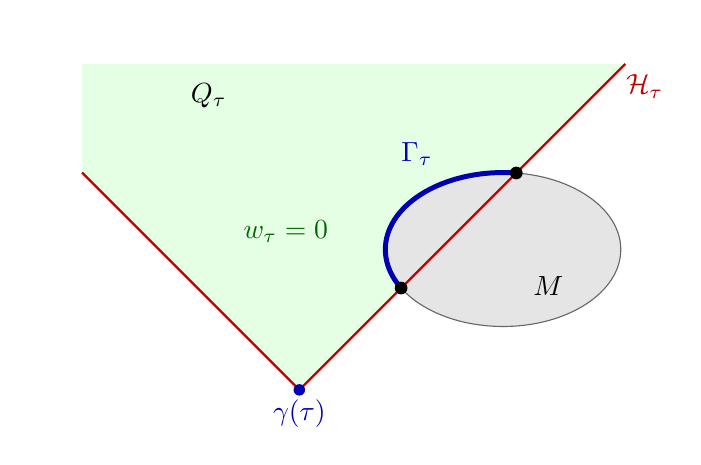
\begin{tikzpicture}[scale=1.15]
% Q_tau = inside of the cone
\fill[green!10] (0,0) -- (3.6,3.6) -- (-2.4,3.6) -- (-2.4,2.4) -- cycle;
% M
\path[name path=ellA] (2.25,1.55) ellipse[x radius=1.3, y radius=0.85];
\fill[gray!20] (2.25,1.55) ellipse[x radius=1.3, y radius=0.85];
\draw[black!60] (2.25,1.55) ellipse[x radius=1.3, y radius=0.85];
% Gamma_tau: the part of the boundary of M in the closure of Q_tau
\begin{scope}
  \clip (0,0) -- (4,4) -- (-3,4) -- (-3,3) -- cycle;
  \draw[blue!70!black, line width=1.8pt] (2.25,1.55) ellipse[x radius=1.3, y radius=0.85];
\end{scope}
% the leaf H_tau
\path[name path=rayA] (0,0) -- (3.6,3.6);
\draw[red!75!black, thick] (-2.4,2.4) -- (0,0) -- (3.6,3.6);
\fill[name intersections={of=ellA and rayA, name=iA}]
  (iA-1) circle (2pt) (iA-2) circle (2pt);
% vertex
\fill[blue!70!black] (0,0) circle (1.8pt);
\node[blue!70!black, below] at (0,0) {$\gamma(\tau)$};
% labels
\node[red!75!black, right] at (3.5,3.35) {$\mathcal H_\tau$};
\node at (-1.0,3.25) {$Q_\tau$};
\node[green!40!black] at (-0.15,1.75) {$w_\tau=0$};
\node at (2.75,1.15) {$\uu$};
\node[blue!70!black] at (1.3,2.6) {$\Gamma_\tau$};
\end{tikzpicture}
\caption{End of the proof of Theorem~\ref{thm_calderon}, for $\tau\in\mathcal R$. The waves agree outside $\overline\uu$, so $w_\tau$ and $dw_\tau$ vanish on the shaded set $Q_\tau\setminus\overline\uu$, hence on $\Gamma_\tau$.}
\label{fig:gamma_density}
\end{figure}

\begin{proof}[Proof of Theorem~\ref{thm_calderon}]
Fix a null-cone extension $(\M,\tilde g)$ of $(\uu,g)$, write $g$ for $\tilde g$, and extend $q_1,q_2$ by zero. Inclusions between Cauchy data sets do not depend on the reference Riemannian metric in \eqref{eq_cds}. Indeed, changing it replaces $\partial_\nu u$ by $a\,\partial_\nu u+Y(u|_{\partial\uu})$, with $a>0$ a function and $Y$ a vector field tangent to $\partial\uu$, and this is the same bijection on both sets. So we may take the reference metric to be $h$. Both $q_j$ are admissible for $A=\max_j\|q_j\|_{C^k}$. Choose $\chi$ as in Lemma~\ref{lem_exterior_source}, so that $\supp\chi\cap\overline\uu=\emptyset$, and let $\tau\in\mathcal R$.

We first show that the two waves agree outside $\overline\uu$:
\[
V_{q_1,\tau}=V_{q_2,\tau}\qquad\text{in }\D\setminus\overline\uu .
\]
Approximate $\chi\,\delta'(\varphi_\tau)$ in $\mathcal E'(\D)$ by smooth sources supported in $\supp\chi\subset\D\setminus\overline\uu$, for instance $\chi\,\eta_\varepsilon'(\varphi_\tau)$ with $\eta_\varepsilon$ a mollifier. Lemma~\ref{lem_gluing} applies to each of them, and passes to the limit by continuity of the retarded solution operators~\cite{bar2007}.

On $Q_\tau$ we have $H(\varphi_\tau)=1$ and $\delta(\varphi_\tau)=0$, so $V_{q_j,\tau}=v_{j,\tau}$ there by \eqref{eq:main}. Hence
\[
w_\tau=v_{1,\tau}-v_{2,\tau}=0\qquad\text{on }Q_\tau\setminus\overline\uu .
\]
By continuity, $w_\tau$ and $dw_\tau$ vanish on the closure of $Q_\tau\setminus\overline\uu$ and we get (see Figure~\ref{fig:gamma_density})
\[
w_\tau=0,\qquad \partial_\nu w_\tau=0,\qquad \nabla_h^{\tan}w_\tau=0\qquad\text{on }\Gamma_\tau .
\]
Thus $E_\tau=0$ for every $\tau\in\mathcal R$, so $\mathcal E=0$, and Theorem~\ref{thm_main} gives $q_1=q_2$.
\end{proof}







\appendix



\section{Facts from Lorentzian Geometry}\label{ap_lorentz}

For an introduction to Lorentzian geometry we refer to~\cite{oneill1983, ringstrom2009}. We consider $(\M, g)$ a connected Lorentzian manifold of dimension $1+n$ with signature $(-,+,...,+)$. A vector $v \in T_p \M \backslash \{0\}, \: p \in \M$, is timelike, spacelike or null if
\begin{equation}
    g(v,v)<0,\quad g(v,v)>0, \quad g(v,v)=0,
\end{equation}
respectively. We say that $v \in T_p \M \backslash \{0\} $ is a causal vector if it is timelike or null, that is $g(v,v) \leq 0$. The manifold $(\M, g)$ will be assumed to be time oriented. That means that there exists a vector field $T$ such that $T(p)$ is timelike for all $p \in \M$. This implies that for a causal vector $v$ one has $g(v,T)<0$ or $g(v,T)>0$. Then $v$ is said to be future-directed if $g(v,T)<0$ and past-directed if the opposite inequality holds.

 A submanifold $S$ of $\M$ is called spacelike if all the non-zero tangent vectors of $S$ are spacelike. A smooth curve $\gamma$ is timelike if its tangent vector $\dot \gamma(s)$ is timelike for all $s \in [a,b]$ with analogous definitions for spacelike, null, causal and future/past directed.

Given $p,q \in \M$ we can define the~\textit{causality relations} on $\M$ as follows.
\begin{enumerate}
    \item  We write $p \leq q$ if $p=q$ or there is a future-directed \textit{causal} curve from $p$ to $q$.

    \item We write $p \ll q$ if there is a future-directed \textit{timelike} curve from $p$ to $q$.
\end{enumerate}





This allows to define the~\textit{causal future} of a subset $A \subset \M$ as the set
\begin{equation}
    J^+(A)=\{q \in \M \textnormal{: there is $p$} \in A \textnormal{ such that } p\leq q \},
\end{equation}
as well as the~\textit{chronological future} of $A \subset \M$ as
\begin{equation}
    I^+(A)=\{q \in \M \textnormal{: there is $p$} \in A \textnormal{ such that } p\ll q \}.
\end{equation}



 We have analogous definitions for the~\textit{causal past} and~\textit{chronological past} $J^-(A)$ and $I^{-}(A)$ of $A$ by reversing the sign of the inequalities above. We write $J^{\pm}(p)= J^{\pm}(\{p\})$ and $I^{\pm}(p)= I^{\pm}(\{p\})$ for points $p \in \M$. The sets $I^{\pm}(A)$ are always open in $\M$. However, $J^{\pm}(A)$ need not be closed.

 We now define global hyperbolicity.
\begin{definition}
    The manifold $(\M, g)$ is~\textit{globally hyperbolic} if
    \begin{enumerate}
        \item \label{point_one} there is no closed causal curve,

        \item \label{point_two} the causal diamonds $J^+(p) \cap J^-(q)$ are compact sets for all $p, q \in \M$.
    \end{enumerate}
\end{definition}



We refer to~\cite{hounnonkpe2019} for this relatively recent definition. If $n \geq 2$ and $\M$ is non-compact then~\eqref{point_one} can be omitted from the definition above~\cite{hounnonkpe2019}. On the other hand, globally hyperbolic manifolds are non-compact. Global hyperbolicity has far reaching consequences, which are summarized in the next theorem. A hypersurface $\Sigma \subset \M$ is called a~\textit{Cauchy surface} if every inextendible timelike curve intersects $\Sigma$ exactly once.

\begin{theorem}
\label{prop_of_globhyper}
    The following are equivalent for $(\M, g)$.

\begin{enumerate}
    \item $(\M, g)$ is globally hyperbolic.

    \item There exists a smooth spacelike Cauchy surface in $\M$.

    \item There exists a temporal function, that is a smooth function $\tau : \M \to \R$ that satisfies $g(d \tau,d \tau)<0$, $d \tau $ is future-directed, and all level sets $\Sigma_t=\tau^{-1}(t)$ are smooth spacelike Cauchy surfaces. The function $\tau$ can be taken surjective and such that its restriction to any inextendible future-directed causal curve is strictly increasing and surjective onto $\R$. Moreover, $\M$ is diffeomorphic to $\R \times \Sigma$ via  $F :\R \times \Sigma_0 \to \M$ with
    \begin{equation}
        (F^*g)(t,x)=c(t,x)(-dt^2+h_t(x)),
    \end{equation}
 where $c>0$ is smooth, $h_t(x)$ is a Riemannian metric on $\Sigma_0$ smoothly depending on $t$ and $t=\tau$.
\end{enumerate}
\end{theorem}
We note that the diffeomorphism $F$ is obtained by flowing $\Sigma_0$ along $-\nabla^{g} \tau$, where $\nabla^{g}$ denotes the gradient operator on $(\M, g).$



This equivalence has been established in~\cite{bernal2003, bernal2005}. See also the references in~\cite[Proposition 2.3]{oksanen2024rigiditylorentziancalderonproblem} from which comes the formulation in Theorem~\ref{prop_of_globhyper}.

\medskip

Globally hyperbolic manifolds provide with a general geometric setting in which the Cauchy problem for the wave equation is well posed. This is the content of the following proposition.
\begin{proposition}
\label{prop_wave_lorentz}
  Let $(\M, g)$ be globally hyperbolic and $P$ a normally hyperbolic operator. Then for any $F \in \mathcal{E}^\prime(\M)$ there exists a unique $u \in \mathcal{D}^\prime (\M)$ such that
 \begin{equation}
\begin{cases}
    P u=F  \quad \textnormal{in } \M,\\
    \supp (u) \subset J^+(\supp (F)).
    \end{cases}
\end{equation}
\end{proposition}
For the existence part of the above proposition we refer to~\cite[Theorem 3.3.1]{bar2007} and the uniqueness follows from~\cite[Theorem 3.1.1]{bar2007}. See as well~\cite[Theorem 6.3.1]{friedlander1976wave}. An operator $P: C^\infty(\M) \to C^\infty(\M) $ with $\M$ a \textit{Lorentzian manifold} is called normally hyperbolic if its principal symbol is given by the metric
\begin{equation}
    \sigma_P(\xi)=g^{-1}(\xi,\xi).
\end{equation}
In particular $P=\bg+q$ with $q \in C^\infty(\M)$ is normally hyperbolic.




\subsection{Auxiliary Riemannian metric}

\begin{lemma}
\label{lem_aux_riem_metric}
Let $(\M,g)$ be a Lorentzian manifold and let $t : \M \to \mathbb{R}$ be a smooth time function such that $\nabla t$ is everywhere timelike.
Define the symmetric $2$-tensor
\[
h(u,v) = g(u,v) + 2\, g(u, T) g(v, T),
\quad \text{where } T = \frac{\nabla t}{\sqrt{-g(\nabla t,\nabla t)}}.
\]
Then $h$ is a Riemannian metric on $\M$. Moreover, the density function associated to $h$ is the same as the density of $g$, that is $d V_h=d V_g=\sqrt{|\det(g_{ij})|}\, dx^0 \wedge \cdots \wedge dx^n$.
\end{lemma}

\begin{proof}
Let $p \in \M$. Since $T$ is timelike we have a direct sum
\[
T_p \M = \mathrm{span}\{T\} \oplus  T^\perp.
\]
We can now choose a $g$-orthonormal frame $\{T, e_1, \dots, e_n\}$ at $p$, so that the matrix of $g$ in this frame is
\[
(g_{ij}) = \mathrm{diag}(-1,1,\dots,1).
\]
We have $g(e_i,T)=0$ for $i \ge 1$ and
\[
h(T,T) = g(T,T) + 2 g(T,T)^2 = -1 + 2 = 1,
\]
\[
h(T,e_i) = 0,
\quad
h(e_i,e_j) = g(e_i,e_j) = \delta_{ij}.
\]
Thus the matrix of $h$ in this frame is
\[
(h_{ij}) = \mathrm{diag}(1,1,\dots,1).
\]
so $h$ is positive definite and therefore a Riemannian metric.
This proves the lemma, since both properties are independent of the choice of frame.
\end{proof}


\subsection{Static and null-cone foliation}

\begin{lemma}[Null-cone foliation in the ultrastatic case]
\label{lem:ultrastatic-foliation}
Let $(N,h)$ be a complete Riemannian manifold and $x_0\in N$ a point
at which $\exp_{x_0}\colon T_{x_0}N\to N$ is a diffeomorphism.
Consider the ultrastatic spacetime $(\mathcal{M},g)=(\mathbb{R}\times N,-dt^2+h)$
and let $K\subset\uu\subset\mathcal{M}$, with $K$ compact and $\uu$ open with compact closure, such that $x_0\notin\pi_N(\overline\uu)$,
where $\pi_N\colon\mathbb{R}\times N\to N$ is the spatial projection.
Then Assumption~\ref{assumption_null_cone_foliation} is satisfied with
$\gamma(\tau)=(\tau,x_0)$ and $f(t,x)=t-d_h(x_0,x)$.
\end{lemma}

\begin{proof}
Since $\overline\uu$ is compact, we may choose
$t_-<t_+$ such that $\overline\uu\subset\mathcal{D}:=I^+(p_-)\cap I^-(p_+)$ with
$p_\pm=(t_\pm,x_0)$.
The diamond can be expressed as
\[
  \mathcal{D}=\bigl\{(t,x):d_h(x_0,x)<\min(t-t_-,\,t_+-t)\bigr\}.
\]
Define $I=(t_-,t_+)$. Then $K\subset\uu\Subset\D$, and $\overline{\uu}\cap\gamma(I)=\emptyset$ since $x_0\notin\pi_N(\overline\uu)$. We now verify the requirements of Assumption~\ref{assumption_null_cone_foliation} for $f(t,x):=t-d_h(x_0,x)$. Since $\exp_{x_0}$ is a global diffeomorphism $d_h(x_0,\cdot)\in C^\infty(N\setminus\{x_0\})$ and $f\in C^\infty(\dg)$. We also have
\[
  g^{-1}(df,df)
  =-(\partial_t f)^2+|\nabla_h d_h(x_0,\cdot)|_h^2,
  =-1+1=0,
\]
since $|\nabla_h d_h(x_0,\cdot)|_h=1$ on $N\setminus\{x_0\}$. Hence, the level sets of $f$ are null hypersurfaces and they clearly foliate $\D$.

The description of the null cones emanating from $\gamma$ is a consequence of the expression
\[
J^+(\gamma(\tau))
=
\{(t,x):d_h(x_0,x)\leq t-\tau\}.
\]
For the inclusion ``$\subset$'', let $(t,x)\in J^+(\gamma(\tau))$ and let
$[0,1] \ni s \to \Gamma(s)=(t(s),x(s))$ be a future-directed causal curve from
$(\tau,x_0)$ to $(t,x)$. Then
\[
0\geq g(\dot\Gamma,\dot\Gamma)
=-\dot t^2+|\dot x|_h^2,
\]
and $\dot t>0$, so $|\dot x|_h\leq\dot t$. Hence
\[
d_h(x_0,x) \leq
\int_0^1 |\dot x|_h\,ds
\leq\int_0^1 \dot t\,ds
=t-\tau.
\]
Conversely, suppose that
\[
d_h(x_0,x)\leq t-\tau.
\]
By completeness of $(N,h)$, there exists a unit-speed minimizing
geodesic $\sigma:[0,L]\to N$ from $x_0$ to $x$, where
$L=d_h(x_0,x)$. Let
\[
\Gamma(s)=
\left(\tau+\frac{t-\tau}{L}s,\sigma(s)\right),
\qquad 0\leq s\leq L.
\]
Then $\Gamma$ joins $(\tau,x_0)$ to $(t,x)$ and
\[
g(\dot\Gamma,\dot\Gamma)
=-\left(\frac{t-\tau}{L}\right)^2+1\leq0,
\]
while $\dot t>0$. Thus $\Gamma$ is future-directed causal, and
$(t,x)\in J^+(\gamma(\tau))$.
\end{proof}

\begin{figure}[ht]
\centering
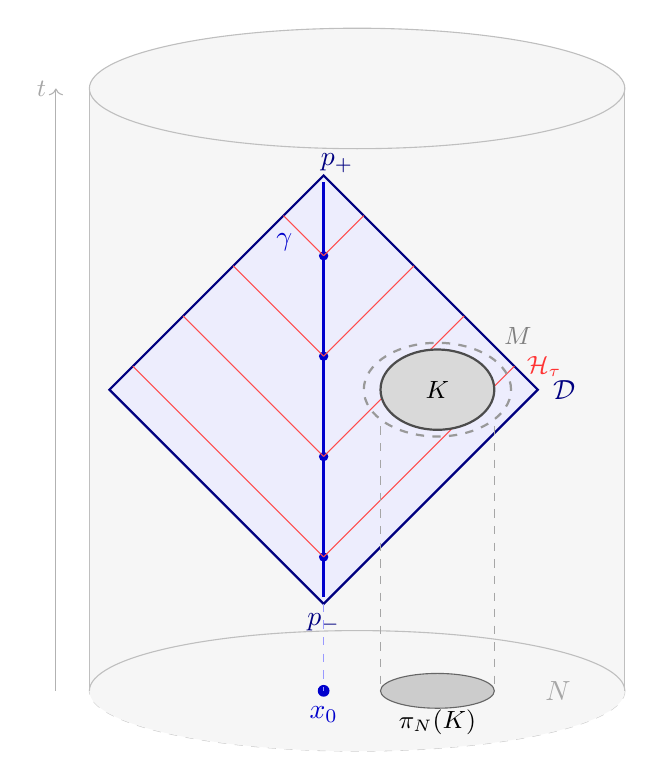
\begin{tikzpicture}[scale=0.85]

% --- Cylinder setup ---
% Base ellipse: center (0, -4.5), rx=4, ry=0.9
% Top  ellipse: center (0,  4.5), rx=4, ry=0.9
% Sides: x = -4 and x = 4, from T=-4.5 to T=4.5

% Back half of base ellipse (dashed)
\draw[gray!40, dashed, thin]
    (0,-4.5) ++(0:4 and 0.9) arc(0:-180:4 and 0.9);

% Fill the interior of the cylinder lightly
\fill[gray!7]
    (-4,-4.5) -- (-4,4.5)
    arc(180:0:4 and 0.9)
    -- (4,-4.5)
    arc(0:-180:4 and 0.9)
    -- cycle;

% Cylinder sides
\draw[gray!50, thin] (-4,-4.5) -- (-4, 4.5);
\draw[gray!50, thin] ( 4,-4.5) -- ( 4, 4.5);

% Top ellipse (full, solid)
\draw[gray!50, thin] (0,4.5) ellipse (4 and 0.9);

% Front half of base ellipse (solid)
\draw[gray!50, thin]
    (0,-4.5) ++(0:4 and 0.9) arc(0:180:4 and 0.9);

% Label N on the base
\node[gray!70] at (3.0, -4.5) {$N$};

% ------------------------------------------------------------------
% gamma at x=-0.5, half-height=3.2 (enlarged diamond).
% p_- = (-0.5,-3.2), p_+ = (-0.5,3.2).
% Right tip: (2.7, 0).  Left tip: (-3.7, 0).
% Edges:
%   bottom-right: t = x - 2.7   (slope +1)
%   right-top:    t = 2.7 - x   (slope -1)
%   top-left:     t = x + 3.7   (slope +1)
%   bottom-left:  t = -x - 3.7  (slope -1)
%
% Right ray from (-0.5,tau): hits right-top t=2.7-x at x=(2.2-tau)/2, t=1.6+tau/2.
% Left  ray from (-0.5,tau): hits left-top  t=x+3.7 at x=(tau-4.2)/2, t=tau/2+1.6.
%
% tau=-2.5: right (2.35, 0.35), left (-3.35, 0.35)
% tau=-1.0: right (1.6,  1.1),  left (-2.6,  1.1)
% tau= 0.5: right (0.85, 1.85), left (-1.85, 1.85)
% tau= 2.0: right (0.1,  2.6),  left (-1.1,  2.6)
% ------------------------------------------------------------------

\fill[blue!8, opacity=0.8]
    (-0.5,-3.2) -- (2.7,0) -- (-0.5,3.2) -- (-3.7,0) -- cycle;
\draw[blue!50!black, thick]
    (-0.5,-3.2) -- (2.7,0) -- (-0.5,3.2) -- (-3.7,0) -- cycle;

\node[blue!50!black, right=2pt] at (2.7,0) {$\mathcal{D}$};
\node[above, blue!50!black] at (-0.3,3.1) {$p_+$};
\node[below, blue!50!black] at (-0.5,-3.2) {$p_-$};

% ------------------------------------------------------------------
% Timelike curve gamma at x=-0.5
% ------------------------------------------------------------------
\draw[blue!80!black, very thick] (-0.5,-3.1) -- (-0.5,3.1);
\node[blue!80!black, left=3pt] at (-0.7, 2.2) {$\gamma$};

\foreach \t in {-2.5,-1.0,0.5,2.0} {
    \fill[blue!80!black] (-0.5,\t) circle (2pt);
}


% ------------------------------------------------------------------
% Null rays
% ------------------------------------------------------------------
% tau=-2.5
\draw[red!70, thin] (-0.5,-2.5) -- (2.35, 0.35);
\draw[red!70, thin] (-0.5,-2.5) -- (-3.35, 0.35);
% tau=-1.0
\draw[red!70, thin] (-0.5,-1.0) -- (1.6, 1.1);
\draw[red!70, thin] (-0.5,-1.0) -- (-2.6, 1.1);
% tau=0.5
\draw[red!70, thin] (-0.5, 0.5) -- (0.85, 1.85);
\draw[red!70, thin] (-0.5, 0.5) -- (-1.85, 1.85);
% tau=2.0
\draw[red!70, thin] (-0.5, 2.0) -- (0.1,  2.6);
\draw[red!70, thin] (-0.5, 2.0) -- (-1.1, 2.6);

% Label
\node[red!80, right=1pt] at (2.35,0.35) {\small$\mathcal{H}_\tau$};

% ------------------------------------------------------------------
% Compact set K: inside diamond, to the right of gamma
% centered at (1.2, 0), enlarged
% ------------------------------------------------------------------
\fill[black!15, draw=black!70, thick]
    (1.2,0) ellipse (0.85 and 0.60);
\node at (1.2,0) {\small$K$};

% Neighbourhood U (dashed)
\draw[black!40, dashed, thick]
    (1.2,0) ellipse (1.1 and 0.7);
\node[black!50] at (2.4,0.80) {\small$\uu$};

% ------------------------------------------------------------------
% Projection of K onto N base
% ------------------------------------------------------------------
\draw[black!35, dashed] (0.35, -0.55) -- (0.35, -4.5);
\draw[black!35, dashed] (2.05, -0.55) -- (2.05, -4.5);

\fill[black!20, draw=black!60]
    (1.2,-4.5) ellipse (0.85 and 0.26);
\node[below=1pt] at (1.2,-4.6) {\small$\pi_N(K)$};

% ------------------------------------------------------------------
% x_0 on the base (below gamma at x=-0.5)
% ------------------------------------------------------------------
\fill[blue!80!black] (-0.5,-4.5) circle (2.5pt);
\node[below=2pt, blue!80!black] at (-0.5,-4.5) {$x_0$};
\draw[blue!40, dashed] (-0.5,-3.2) -- (-0.5,-4.5);

% ------------------------------------------------------------------
% Time axis on the LEFT
% ------------------------------------------------------------------
\draw[->, gray!60, thin] (-4.5,-4.5) -- (-4.5,4.5)
    node[left, gray!70] {\small$t$};

\end{tikzpicture}
\caption{The spacetime $\mathbb{R}\times N$ represented as a cylinder. The null cone foliation assumption~\ref{assumption_null_cone_foliation} is satisfied as soon as there is a point $x_0$ outside of the spatial projection of the compact $K$, such that $\exp_{x_0}$ is a global diffeomorphism.}
\label{fig:ultrastatic-3d}
\end{figure}



\section{Distributions on manifolds}
\label{ap_distrib_manifold}

We collect here some definitions and facts about distributions. We closely follow~\cite[Chapter 6]{hormander1990}. We start by recalling the notion of pullback of distributions, given by~\cite[Theorem 6.1.2]{hormander1990}. This extends the composition operation in the following sense.

Let $U_j \subset \R^{n_j}, j \in \{1,2\}$ be open sets and $f: U_1 \to U_2$ be a smooth map such that $df(x)$ is surjective for every $x \in U_1$. Then there is a unique linear map $f^*: \mathcal{D}^\prime(U_2) \to \mathcal{D}^\prime(U_1)$ such that $f^*u=u \circ f$ when $u$ is smooth, called the pullback of $u$ by $f$. When defined, the pullback satisfies the usual rules of computation. In particular, the chain rule holds
\begin{equation}
\label{eq_chain_rule}
    \partial_j f^*u=\sum_{k=1}^{n_2} (\partial_j f_k) f^* \partial_k u.
\end{equation}
In the case where $f$ is a diffeomorphism, the pullback is given by
\begin{equation}
\label{eq_pull_diffeo}
    (f^*u, \phi)_{\mathcal{D}^\prime(U_1), C^\infty_0(U_1)}=  (u, |\det d(f^{-1})|(\phi \circ f^{-1}))_{\mathcal{D}^\prime (U_2), C^\infty_0(U_2)}.
\end{equation}

\bigskip

In an arbitrary manifold $M$, there is not a canonic way of integrating. As a consequence, there is no natural embedding of a smooth function $u$ in the dual of $C^\infty_0(M)$ via $\phi \to \int u\phi$,  since $\int u \phi$ does not have an invariant meaning. The space $\mathcal{D}^\prime (M)$ of distributions on $M$ is instead defined by gluing together distributions $u_\kappa \in \mathcal{D}^\prime (\kappa(U_\kappa))$, given in local coordinates $(U_\kappa, \kappa )$, such that
\begin{equation}
\label{eq_trans_law_distrib}
    u_{\kappa^\prime}=(\kappa \circ \kappa^{\prime -1})^* u_\kappa \textnormal{ in } \kappa^\prime(U_\kappa \cap U_{\kappa^\prime}),
\end{equation}
holds on an overlapping chart.



As for the dual of $C^\infty_0(M)$, it can be identified with the space of~\textit{distribution densities} on $M$. Those are obtained by gluing together distributions $u_\kappa \in \mathcal{D}^\prime (\kappa(U_\kappa))$, given in local coordinates $(U_\kappa, \kappa )$, but satisfying a different transformation law
\begin{equation}
\label{eq_trans_law_density}
    u_{\kappa^\prime}=|\det d \psi| \psi ^* u_\kappa \textnormal{ in } \kappa^\prime(U_\kappa \cap U_{\kappa^\prime}), \quad \psi=\kappa \circ \kappa^{\prime -1},
\end{equation}
on an overlapping chart. Now given $u$ a distribution density on $M$ and $\phi \in C^\infty_0 (U_\kappa)$ supported on a coordinate neighborhood, we define the pairing
\begin{equation}
    (u, \phi)=(u_\kappa, \phi \circ \kappa^{-1})_{\mathcal{D}^\prime(\kappa(U_\kappa)), C^\infty_0 (\kappa(U_\kappa))},
\end{equation}
and this can be extended to any $\phi \in C^\infty_0(M)$ by using a partition of unity subordinate to a system of coordinates.  The transformation law~\eqref{eq_trans_law_density} ensures that $(u, \phi)$ is well defined. Indeed, we consider an overlapping chart $U_\kappa \cap U_{\kappa^\prime}$ and we write $U_1=\kappa^\prime (U_\kappa \cap U_{\kappa^\prime})$ and $U_2=\kappa (U_\kappa \cap U_{\kappa^\prime})$. Using~\eqref{eq_trans_law_density} and the pullback expression~\eqref{eq_pull_diffeo} we find
\begin{align}
    &(u_{\kappa^\prime}, \phi \circ \kappa^{\prime -1})_{\mathcal{D}^\prime(U_1), C^\infty_0 (U_1)}=(|\det d \psi| \psi ^* u_\kappa,\phi \circ \kappa^{\prime -1} )_{\mathcal{D}^\prime(U_1), C^\infty_0 (U_1)} \\
    &=( \psi ^* u_\kappa,|\det d \psi| (\phi \circ \kappa^{\prime -1} ))_{\mathcal{D}^\prime(U_1), C^\infty_0 (U_1)}\\&
    =( u_\kappa,|\det d \psi^{-1}| ( |\det d \psi| \circ \psi^{-1} )(\phi \circ \kappa^{ -1} ))_{\mathcal{D}^\prime(U_2), C^\infty_0 (U_2)} =(u_{\kappa}, \phi \circ \kappa^{-1})_{\mathcal{D}^\prime(U_2), C^\infty_0 (U_2)}.
\end{align}

We notice finally that if $\phi$ is a smooth compactly supported density and $u$ a distribution then $\phi u$ is a distribution density.  This identifies $\mathcal{D}^\prime (M)$ with the dual of smooth compactly supported densities by associating to a distribution $u$ the functional $\phi \to (u \phi, \chi )$ with $\chi=1$ on the support of $\phi$.

\bigskip

Now suppose $\mu$ is a fixed given density on $M$. The map
\begin{equation}
    u \to \mu u,
\end{equation}
allows to identify distributions with distributions densities and functions with densities. In particular, in a semi-Riemannian manifold $(M, g)$ endowed with its canonical density $\mu= |\mathrm{vol}_g| = \sqrt{|\det(g_{ij})|}\, |dx^1 \wedge \cdots \wedge dx^n|$ we have the identification $\mathcal{D}^\prime (M) = (C^\infty_0(M))^\prime$ by identifying a distribution $T \in  \mathcal{D}^\prime (M)$ with the functional $\phi \to (T, \phi \mu)$. In other words, once a density has been fixed on $M$ we have for $T \in  \mathcal{D}^\prime (M)$ the following dictionary
\begin{equation}
    (T, \phi)_{\mathcal{D}^\prime (M), C^\infty_0(M)}=(T , \phi \mu)=(\mu T, \phi).
\end{equation}
In the second equality $T$ is interpreted  as an element of the dual space of smooth compactly supported densities. In the last one we have a pairing between a distribution density and a smooth compactly supported function.

Now consider $(M,g)$ a semi-Riemannian manifold with its canonical density $\mu$ and $P$ a differential operator acting on functions $P: C^\infty(M) \to C^\infty(M)$. The action of $P$ extends to densities via conjugation by $\mu$. That is, for a density $\omega $ we define the density $P \omega$ as
\begin{equation}
    P \omega= \mu P(\mu^{-1}\omega),
\end{equation}
where $\mu^{-1} \omega$ is a smooth function on $M$.

Unwinding the definitions and identifications above we see that given a distribution $T \in \mathcal{D}^\prime(M)$ the distribution $PT \in \mathcal{D}^\prime (M) $ is well defined and acts on functions $\phi \in C^\infty_0(M)$ by
\begin{equation}
    (PT, \phi)=(T, P^*_\mu \phi),
\end{equation}
where the operator $P^*_\mu$ is the formal adjoint of $P$ for the density $\mu$, given by
$$
\int (Pf) g \mu = \int f (P^*_\mu g) \mu, \textnormal{ for } f,g \in C^\infty_0(M).
$$
In particular, one has the expected identity for the Laplace--Beltrami operator on $M$ and a distribution $T \in \mathcal{D}^\prime(M)$
\begin{equation}
    (\bg T,\phi)=(T, \bg \phi).
\end{equation}




\bibliographystyle{alpha}
\bibliography{master,lorentzian_extra}

\end{document}